\chapter{Editing}%
\label{cha:editing}

Editing comprises both time and track space.  The timeline consists
of the time certain media appear on the track going left to right
and a set of tracks from the top to the bottom.  There are 2 methods
of timeline editing -- drag and drop editing, also called
\textit{arrow mode}, and cut and paste editing or \textit{I-beam
  mode}.  Cut and Paste is the default editing mode.  An additional,
but not often considered editing method is called \textit{two-screen
  editing} where the Viewer is used to view media and then the
desired clip from the media is transferred to the timeline.

The timeline is where all editing decisions are made
(figure~\ref{fig:timeline}).  This is a stack of tracks in the
center of the main window.  It can be scrolled up, down, left and
right with the scrollbars on the right and bottom.  It can also be
scrolled up and down with a mouse wheel, or left and right while
holding down the Ctrl key and using the mouse wheel.

\begin{figure}[htpb]
  \centering
  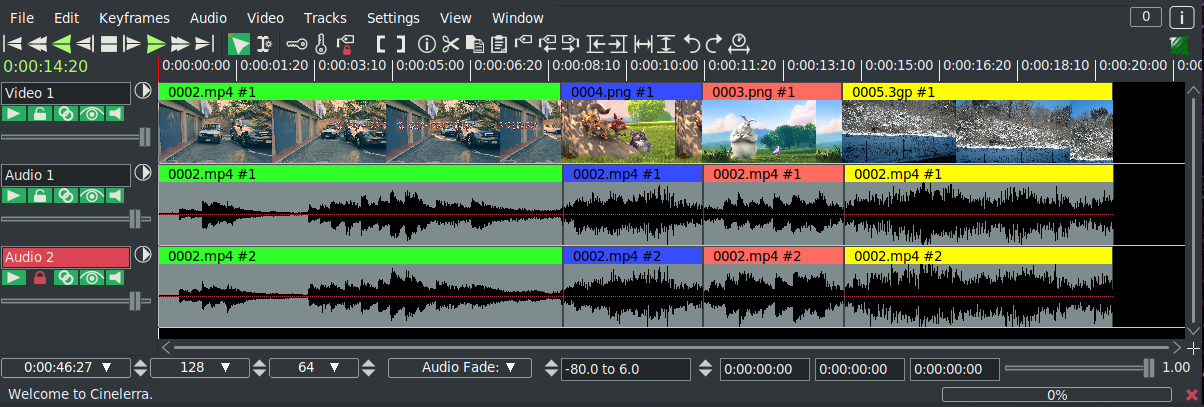
\includegraphics[width=1.0\linewidth]{timeline.png}
  \caption{Timeline editing session}
  \label{fig:timeline}
\end{figure}

The active region is the range of time which is affected by editing
commands on the timeline.  The active region is determined first by
the presence of in/out points on the timeline.
%
If those do not exist the highlighted region is used. To reiterate,
\emph{highlighting} is done in \emph{cut and paste mode} by moving
the insertion point with the mouse in the timeline to where you want
to start. Then hold down the LMB\@, drag the mouse to where you want
the end point to be and release the LMB\@. In \emph{drag and drop
  mode}, the method to create a highlighted selection is to hold
down the Ctrl key and double click with the LMB with the mouse over
that column.

If no highlighted region exists, the insertion point is used as the
start of the active region.  Some commands treat all the space to
the right of the insertion point as active while others treat the
active length as 0 (zero) if no end point for the active region is
defined.

Most importantly, editing decisions never affect source material
meaning that it is non-destructive editing.  So not only does your
original media stay completely untouched, it is much faster than if
you had to copy all the media affected by an edit.  Editing only
affects pointers to source material, so if you want to have a new
modified media file at the end of your editing session which
represents the editing decisions, you need to render it.  Saving and
loading your edit decisions is explained in the Load, Save and the
EDL section and rendering is explained in the section on Rendering.

In the following editing sections, references to common operations
are scattered within any of the modes where they seem pertinent.
However, many of the editing operations work in different modes.


\section{The Patchbay}%
\label{sec:patchbay}

On the left of the timeline is a region known as the patchbay.  The
patchbay enables features specific to each track as described next.


\begin{description}
\item[Textbox] for naming the track.  The default names will usually
  be Video \#, Audio \#, or Mixer \# if using the multi-camera/mixer
  operations.  A \# will be designated for subsequent tracks as in 1,
  2, 3 and so on.
\item[Expander] which is a down arrow on the right side, is for
  viewing more options on the patchbay and for viewing the effects
  represented on the track.  You can just click on the expander to
  expand or collapse the patchbay and the track.  If it is pointing
  sideways, the track is collapsed.  If it is pointing down, the track
  is expanded.  Existing effects appear below the media for the track.
\end{description}

Below the textbox name are several toggles referred to as
\textit{attributes} for different features (currently there are 5 as
shown in figure~\ref{fig:patchbay01}).  If the toggle button is
shadowed by a color, the feature is enabled. If the toggle is the
background color of most of the window, it is disabled. Click on the
toggle to enable/disable the feature.

\begin{wrapfigure}[16]{O}{0.3\linewidth}
  %\vspace{-2ex}
  \centering
  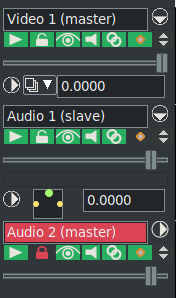
\includegraphics[width=0.79\linewidth]{patchbay01.png}
  \caption{Patchbay}
  \label{fig:patchbay01}
\end{wrapfigure}

Several mouse operations speed up the configuration of several
tracks at a time. Click on an attribute and drag the cursor across
adjacent tracks to copy the same attribute to those tracks.  Hold
down Shift while clicking a track's attribute to enable the
attribute in the current track and toggle the attribute in all the
other tracks. Or you can:

\begin{enumerate}
\item hold down Shift while clicking an attribute,
\item click until all the tracks except the selected one are
  disabled,
\item then drag the cursor over the adjacent track to enable the
  attribute in the adjacent track.
\end{enumerate}

The 5 \textit{attributes} are described here next followed by the other available feature icons and their description.

\begin{description}
\item[Play Track] determines whether the track is rendered or
  not. If it is off, the track is not rendered.  For example if you
  turn it off in all the video tracks, the rendered media file will
  have only audio tracks.  If the track is chained to any other tracks
  by a shared track effect, the other tracks perform all the effects
  in this shared track, regardless of play status of the shared track
  that in this particular case affects the media output but not fade
  and effects.
\item[Arm Track] determines whether the track is armed or not.
  Only the armed tracks are affected by editing operations. Make sure
  you have enough armed destination tracks when you paste or splice
  material or some tracks in the material will get left out.  In
  addition to restricting editing operations, the armed tracks in
  combination with the active region determine where material is
  inserted when loading files.  If the files are loaded with one of
  the insertion strategies which do not delete the existing project,
  the armed tracks will be used as destination tracks.
\end{description}

\begin{description}
\item[Gang Fader] cause the fader to track the movement of
  whatever other fader you are adjusting by dragging either the fader
  or the curve on the track.  It doesn't affect the editing made with
  menu controls.  A fader is only ganged if the arm track is also on.
  This is often used to adjust audio levels on all the tracks
  simultaneously.  Gang also causes Nudge parameters to synchronize
  across all the ganged tracks.
\item[Draw Media] determines if picons or waveforms are drawn on
  the asset in the track.  You may want to disable this if you know
  that the media/format takes a long time to draw on the timeline.  By
  default it is set to on in order to see picons on the timeline.
\item[Don’t send to output] -- more commonly called
  \textit{mute} -- causes the output to be thrown away once the track is
  completely rendered. This happens whether or not \textit{Play track}
  is on.  For example if you mute all the video tracks, the rendered
  media file will have a blank video track.  Mute track is represented
  on the timeline with a line that has the default color of a
  pinkish-orange.  Use the pulldown \texttt{View $\rightarrow$ Mute} to
  have the line displayed.  It is a keyframable attribute, but Mute
  track keyframing is a toggle and it has only the two values of on or
  off. If a track is part of a shared track effect, the output of the
  track with the shared track effect is overlaid on the final output
  even though it is routed back to another track (the shared track).
  Mute track is used to keep the track with the shared track effect
  from overlapping the output of the source track (the shared track)
  where the shared track effect is not present.
\item[Track Data Height] this up/down toggle symbol to the immediate right
of the 5 attributes, is used to individually resize each track.  This makes
it very easy to temporarily expand or contract the size of that track either
by clickin with the left mouse button or using the middle wheel up/down.
\item[Fader slider] fade values are represented on the timeline
  with a pink (default color) curve that is keyframable.  All tracks have a fader, but
  the units of each fader depend on whether it is audio or video.
  Audio fade values are in dB. They represent relative levels, where 0
  is the unaltered original sound level, -40 is silence, -80 the
  minimum value set by default.  You can move fader and keyframes down
  to -80 but the parameter's curve won't go below -40.  For your
  convenience you can set a different fade range with the curve zoom.
  Audio fader’s main purpose is to \textit{fade out} sound or to lower
  the sound level smoothly to silence, or \textit{fade in} to make
  sounds appear gradually instead of suddenly.  Video fade values are
  the percentage of opacity of the image in normal overlay mode, the
  percentage of the layer that is mixed into the render pipeline in
  the other overlay modes.  Click and drag the fader to fade the track
  in and out.  If it is ganged to other tracks of the same media type,
  with the arm option enabled, the other faders should follow.  Hold
  down the Shift key and drag a fader to center it on the original
  source value (0 for audio, 100 for video).
\item[Mixer] in the expanded patchbay for that track designates
  the multi-camera mixer mode.
\item[Overlay mode] in the expanded patchbay is used for
  porter-duff operations and is full explained in
  \nameref{cha:overlays} chapter.
\item[Nudge] is in the expanded patchbay.  The nudge value is
  the amount the track is shifted left or right during playback. The
  track is not displayed shifted on the timeline, but it is shifted
  when it is played back. This is useful for synchronizing audio with
  video, creating fake stereo, or compensating for an effect which
  shifts time, all without altering any edits
  (figure~\ref{fig:overlay}).

  \begin{figure}[htpb] \centering
    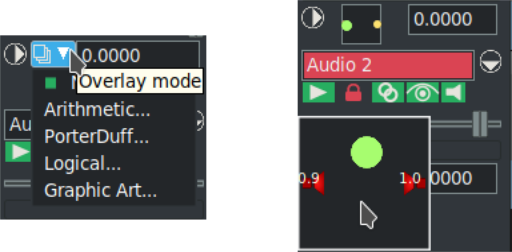
\includegraphics[width=0.65\linewidth]{overlay.png}
    \caption{Video Overlay, audio Pan and Nudge.}
    \label{fig:overlay}
  \end{figure}

  Enter the amount of time to shift to instantly shift the
  track. Negative numbers make the track play later. Positive numbers
  make the track play sooner. The nudge units are either seconds or
  the native units for the track (frames or samples). Select the units
  by right clicking on the nudge textbox and using the context
  sensitive menu. Nudge settings are ganged with the Gang faders
  toggle and the Arm track toggle. Use the mouse wheel over the nudge
  textbox to increment and decrement the value.
\item[Pan] is available in the expanded patchbay for audio
  tracks via a panning box. Position the pointer in the panning box
  and click/drag to reposition the audio output among the speaker
  arrangement. The loudness of each speaker is printed on the relative
  icon during the dragging operation. The panning box uses a special
  algorithm to try to allow audio to be focused through one speaker or
  branched between the nearest speakers when more than 2 speakers are
  used.
\end{description}

Press the Tab key while the cursor is anywhere over a track to
toggle the track arming status. Press Shift-Tab while the cursor is
over a track to toggle the arming status of every other track.

\paragraph{Automatic audio mappings} Several convenience functions
are provided for automatically setting the panning to several common
standards. They are listed in the Audio menu. These functions only
affect armed audio tracks. They are:

\begin{description}
\item[Audio~$\rightarrow$~Map 1:1] This maps every track to
  its own channel and wraps around when all the channels are
  allocated. It is most useful for making 2 tracks with 2 channels map
  to stereo and for making 6 tracks with 6 channels map to a 6 channel
  sound card.
\item[Audio~$\rightarrow$~Map 5.1:2] This maps 6 tracks to 2
  channels. The project should have 2 channels when using this
  function. Go to \texttt{Settings $\rightarrow$ Format} to set the
  output channels to 2. This is most useful for down-mixing 5.1 audio
  to stereo (for more information refer to Configuration, Settings and
  Preferences section~\ref{sub:audio_out_section}).
\end{description}

\paragraph{Standard audio mappings} Although \CGG{} lets you map any
audio track to any speaker, there are standard mappings you should
use to ensure the media can be played back elsewhere. Also, most
audio encoders require the audio tracks to be mapped to standard
speaker numbers or they will not work.

In the channel position widget, the channels are numbered to
correspond to the output tracks they are rendered to. For stereo,
the source of channel 1 needs to be the left track and the source of
channel 2 needs to be the right track.  For 5.1 surround sound, the
sources of the 6 channels need to be in the order of center, front
left, front right, back left, back right, low frequency effects. If
the right tracks are not mapped to the right speakers, most audio
encoders will not encode the right information if they encode
anything at all. The low frequency effects track specifically can
not store high frequencies in most cases.


\section{Manipulating Tracks}%
\label{sec:manipulating_tracks}

Tracks in \CGG{} either contain audio or video.  There is no special
designation for tracks other than the type of media they contain.
When you create a new project, it contains three default tracks: one
video track and two audio tracks.  You can still add and delete
tracks from the menus.  The Tracks menu contains a number of options
for dealing with multiple tracks simultaneously.  Each track itself
has a popup menu which affects one track.

Operations in the \textbf{Tracks pulldown} affect only tracks which
are armed.

\begin{description}
\item[Move tracks up | Move tracks down] shift all the armed
  tracks up or down the stack.
\item[Delete tracks] deletes the armed tracks.
\item[Delete last track] deletes the last track, whether it is
  armed or not.
\item[Concatenate tracks] operation copies all the assets of
  every disarmed but playable track and concatenates it by pasting
  those assets at the end of the first set of armed tracks. They are
  pasted one after the other, keeping the same order they have on the
  stack. If there are two armed tracks followed by two disarmed
  tracks, the concatenate operation copies the assets of the two
  disarmed tracks and pastes them after the assets of the two armed
  tracks. If there are three disarmed tracks instead, the assets of
  two tracks are pasted after the assets of the armed tracks and the
  assets of the third track are pasted at the end of the first armed
  track. The destination track wraps around until all the disarmed
  tracks are concatenated. Disarmed tracks that are not playable are
  not concatenated.
\item[Append to project] allows for creating new tracks after
  any existing tracks.
\item[Add subttl] will add a track for subtitles at the top of
  the other tracks.
\end{description}

The \textbf{Audio} and \textbf{Video pulldowns} each contain an
option to add a track of their specific type. In the case of audio,
the new track is put on the bottom of the timeline and the output
channel of the audio track is incremented by one. In the case of
video, the new track is put on the top of the timeline. This way,
video has a natural compositing order. New video tracks are overlaid
on top of old tracks.


\section{Two Screen Editing}%
\label{sec:two_screen_editing}

This is a fast way to construct a program out of movie files (in
other programs is called \textit{three points editing}). The idea
consists of viewing a movie file in one window and viewing the
program in another window. Subsections of the movie file are defined
in the viewer window and transferred to the end of the program in
the program window.  Two screen editing can be done simply by using
keyboard shortcuts.  To get familiar with which keys to use, move
the mouse pointer over the transport panel and a tooltip appears,
showing what key is bound to that button.

To begin a two screen editing session, load your media resources by
using the main menu \textbf{File pulldown} and choose \textit{Load
  files}; make sure the insertion mode is set to \textit{Create new
  resources only}.  This insertion strategy is to ensure that the
timeline stays unchanged while new resources are brought in. Go to
the Resources window and select the Media folder. The newly loaded
resources will appear. Double click on a resource or drag it from
the media side of the window over to the Viewer window.

Check to make sure there are enough armed tracks on the timeline to
put the subsections of source material that you want.  Usually this
would be one video track and two audio tracks, but if there are not
enough, just create new tracks or arm more tracks.

Now to start your 2 screen editing, in the viewer window, define a
clip from the media file:

\begin{enumerate}
\item Set the starting point with the In pointer button.  You
  will see a left hand bracket on the timebar.
\item Move your cursor to the ending point of the clip you want
  to use.
\item Set the ending point with the Out pointer right hand
  bracket.
\item You will see a colored bar inside the brackets for easier
  viewing.
\item Drag the In/Out point with the mouse to conveniently
  change their position.
\end{enumerate}

These In/Out points define a clip.  You can now use this in a couple
of different ways.

\paragraph{Splice} The splice icon, or shortcut letter “\texttt{v}”,
inserts the selected area in the timeline after the insertion point.
After the splice has taken effect, the insertion point moves to the
end of the edit ready to be used as the next splice location. This
way you can continuously build up the program by splicing.  If an In
point or an Out point exists on the timeline the clip is inserted
after the In point or after the Out point. If both In and Out points
are set on the timeline, the clip is inserted after the In point. If
there are edits after your chosen splice location on the timeline,
they will be moved to the right.

\paragraph{Overwrite} The overwrite icon, or shortcut letter
“\texttt{b}”, overwrites the region of the timeline after the
insertion point with the clip. If an In point or an Out point exists
on the timeline the clip is overwritten after the In point or after
the Out point. If both In and Out points are set on the timeline,
the clip is inserted after the In point. If a region is highlighted
or both In and Out points exist they limit the region of the
overwriting and the clip may therefore be shortened. Here is a
detailed explanation to take advantage of this method.

To overwrite exactly on a precise region of the timeline:

\begin{enumerate} [noitemsep]
\item Arm only tracks to change.
\item Define the destination region on the timeline with [ and
  ], the In and Out points.
\item You can achieve maximum precision by setting the active
  region in the zoom panel.
\item Define the clip you want to use in the viewer with [ and
  ], the In and Out points.
\item Overwrite from Viewer to the timeline.
\end{enumerate}

If the destination region is shorter than the clip defined in the
viewer, the portion of the clip longer than the destination region
won't be inserted and on the timeline the following edits won't
move.  If the destination region is longer than the clip defined in
the viewer, the destination region will shrink and on the timeline
the following edits will move to the left.

\paragraph{Clip} The clip icon, or shortcut letter “\texttt{i}”,
generates a new clip for the resource window containing the affected
region but does not change the timeline.  Every clip has an
optional/default title and description.

\paragraph{Copy} The copy icon, or shortcut letter “\texttt{c}”,
copies the selection into the copy buffer.

\subsection{Use Case – Working with Sequences}
\label{sub:use_case_working_sequences}

\textit{From the Viewer to the Timeline with the sequences imported
  in a Master Project.}

A convenient methodology for working on a Master project along with
1 or more previously saved Sub projects or \textit{sequences} use
case is described here.  A sequence is an edited assembly of audio
and video clips generally consisting of a series of videos that
relate to the same activity. This use case explains how to work this
way and some things you need to be aware of.

\begin{enumerate}
\item First load your Master project, which you worked on and
  saved earlier as an \texttt{.xml} file, using an Insertion strategy
  of \textit{Replace current project}.  Generally this Master project
  consists of media with any of the attributes of clips, autos,
  possibly keyframes, and effects.  You will see your project on the
  main timeline and the Media files that are part of this Master
  project will be displayed in the Resources window in the Media
  folder.
\item Previously you may have also saved a Sub project, which
  will now be referred to as a Sequence, as an \texttt{.xml} file that
  may contain any of the same such things: media, clips, autos,
  keyframes, effects.  Second you will want to load the Sequence using
  an Insertion strategy of \textit{Create new resources only}.  When
  you do the load, this Sequence will show as a file in the Resources
  window in the Clips folder.  The actual media will show in the Media
  folder.
\item Now Drag and Drop the Sub project from the Clips folder to
  the Viewer.
\item Set In and Out Pointers in the Viewer to the region of
  interest in the Sub project and in the Timeline of the Main window
  of your Master project, move the cursor position to where you would
  like to insert this In/Out section.
\item Click on the \textit{Splice (v)} button in the Viewer to
  insert this section into the Master project timeline.  All of the
  attributes of the selected Sub project section will now be inserted
  in the main timeline to include the autos, keyframes, effects, and
  labels.
\item Alternatively, if you click on the \textit{Overwrite (b)}
  button in the Viewer, you can see the Sub project In/Out section in
  the timeline, but without its autos, effects, keyframes, etc.  If in
  the timeline there were some autos, effects, and keyframes in that
  Master project, they will be in effect for the new section.
\end{enumerate}

You can see the advantages of using Splice versus Overwrite to
either insert (splice) with all of the attributes of a specific
section of your Sequence or to overwrite without the attributes to
allow for the smooth operation on the timeline by retaining the
timeline’s attributes at that point.

NOTE: for correct operation of this use case, you should have the
same (or more) number of tracks in the Master project as you do in
the Sequence.  To avoid having to know how many tracks you need, you
can use the Nest feature as described in the Nesting section
(\ref{sub:nesting}).


\section{Cut and Paste Editing}%
\label{sec:cut_paste_editing}

This is the more traditional method of editing in \CGG{} and
therefore is the default.  To enable the cut and paste editing mode
on the timeline, select the I-beam toggle on the control bar at the
top of the main program window. You can copy edits in the same
track, copy from different tracks in the same instance, start a
second instance of \CGG{} and copy from one instance to the other or
load a media file into the Viewer and copy from there.

To start editing, load some files onto the timeline.  Select a
region of the timeline by click dragging on it and select the cut
button to cut it. Move the insertion point to another point in the
timeline and select the paste button.  Assuming no In/Out points are
defined on the timeline this performs a cut and paste operation.

Most editing operations are listed in the Edit pulldown. Some of
them have a button on the program control toolbar as well as a
keyboard shortcut.  The keyboard shortcut is in parenthesis here.

\begin{description}
\item [Split | Cut] (x) Delete the selected area and put it in
  the cut buffer for future pasting.
\item[Copy] (c) Copy the selected area and put it in the cut
  buffer for future pasting.
\item[Paste] (v) Paste the material that is in the cut buffer.
\item[Clear] (Del) Clear the selected area. If the insertion
  point is over an edit boundary and the edits on each side of the
  edit boundary are the same resource, the edits are combined into one
  edit comprised by the resource. The start of this one edit is the
  start of the first edit and the end of this one edit is the end of
  the second edit. This either results in the edit expanding or
  shrinking.
\item[Paste silence] (Shift+Space) Paste blank audio/video for
  the length of the selected area. Following edits will be pushed to
  the right.
\item[Mute Region] (m) Overwrite blank audio/video on the
  selected area. Following edits don't move.
\item[Trim Selection] Delete everything but the selected region.
\item[Select All] (a) Select the whole timeline.
\end{description}

In Cut and Paste editing mode you can \textit{edit labels} as
well. By enabling Edit labels in the \textbf{Settings pulldown}, or
by disabling the Lock labels from moving button on the Program
Control Tool Bar, labels will be cut, copied or pasted along with
the selected regions of the armed tracks.

Using labels and In/Out points are useful in editing audio.  You can
set In/Out points for the source region of the source waveform and
set labels for the destination region of the destination
waveform. Perform a cut, clear the In/Out points, select the region
between the labels, and perform a paste.

\paragraph{In / Out Points} The In and Out bracket placement is
explained here to illustrate their usage.  Because of the shape of
the markers [ and ] you may assume that they are inclusive -- that
everything placed in between would be included in the clip, such as
in the case of being transferred to the timeline from the Viewer.
In reality, one of the two markers will not include the frame that
was visible at the time the marker was affixed. Depending on whether
the \textit{Always show next frame} option is used or not, it is the
In or Out marker that will not be inclusive.

To obtain a clip on the timeline exactly as you saw in the Viewer,
you must necessarily move the In mark back from the beginning before
the first desired frame or move the Out mark forward after the last
desired frame, depending on the \textit{Always show next frame}
setting.

Some of the confusion can be attributed to the fact that the Viewer
shows frames, while the markers determine spaces, i.e.\ times, that
are not visible between frames. You have to think of each frame as
being delimited by two spaces -- one preceding and one following.
The In mark is always placed before the displayed frame and the Out
mark is always placed after the displayed frame, while taking into
account in its calculations whether the \textit{Always show next
  frame }option is used or not. If you just remember that the
reference of the markers is in the middle of the icon, you will
avoid confusion.

\paragraph{Overwrite} To perform overwriting within the timeline
paste on a selected region (highlighted or between In/Out
points). The selected region will be overwritten. If the clip pasted
from the clipboard is shorter than the selected region, the selected
region will be shrunk. Following edits will move. If the clip pasted
from the clipboard is longer than the selected region, the selected
region will be overwritten with the first part of the clip and the
remaining part of the clip will be written after the
overwriting. Following edits will move.

\paragraph{Tracks $\rightarrow$ Concatenate tracks} This operation
copies all the assets of every disarmed but playable track and
concatenates it by pasting those assets at the end of the first set
of armed tracks. They are pasted one after the other, keeping the
same order they have on the stack.

\paragraph{Split -- blade cut and hard edges:} You can cut the
tracks into 2 pieces on the timeline by putting the hairline cursor
on the place you want to do a cut and then using the character “x”
or the scissors tool (figure~\ref{fig:cut}).

\begin{wrapfigure}[16]{O}{0.3\linewidth}
  \vspace{-2ex}
  \centering
  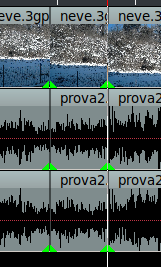
\includegraphics[width=0.9\linewidth]{cut.png}
  \caption{Blade cut}
  \label{fig:cut}
\end{wrapfigure}

A \textit{cut} uses a non-empty selection region, where the
\textit{blade cut} or \textit{split} has no duration in the
selection, just a hairline.  As usual the use of cut when a
selection is set, deletes/cuts the highlighted area.  In the case
where an In point or an Out point exists on the timeline, the clip
is split at the location of the In/Out point since it has priority
over the cursor location.  A blade cut simply splits the edit into
two edits.  In order to have the video and audio aligned, it works
best to have \texttt{Settings $\rightarrow$ Align cursor on
  frames}.  When a blade cut occurs, the edges are created as
\textit{hard edges}.  These are edges that cannot be deleted by
track optimizations.
%
\CGG{} has built-in optimization on the timeline.  So that whenever
two parts on the timeline are sequential frames, it automatically
optimizes by making them into 1 item.  So if you are cutting,
dragging, editing, or whatever and somehow frame \# 40 ends up
right next to frame \# 41, it optimizes them together.  This
optimization affects many areas throughout the program code.  When
you do a blade cut/split, all armed tracks will be included in the
cut and green-colored triangles will show on the bottom of the
track on both the left and the right side of the cut.  This is a
\textit{hard edge} marker toggle, as opposed to the soft edge
designation for an ordinary edit.  The \textit{hard edge} marker
can be toggled off/on if so desired.  In order to not interfere
with the usual drag handles, only a few pixels are used for the
toggle so you have to be sure you have the cursor right over the
hard edge triangle -- when in position, it will be obvious because
you can see an arrow pointing to the corner.  Use Shift-left mouse
button 1 to toggle off/on the hard edge marker on all tracks
simultaneously.


\section{Drag and Drop Editing}%
\label{sec:drag_drop_editing}

To enable the drag and drop editing mode on the timeline, select the
arrow toggle on the control bar at the top of the main program
window.  Drag and drop editing is a quick and simple way of working
in \CGG{}, using mostly only the mouse. The basic idea is to create
a bunch of clips, then drag them in order into the timeline, thus
building prototype media that you can watch in the compositor. If
after watching it, you wish to re-arrange your clips, set effects,
add transitions or insert/delete material, just drag and drop them
on the timeline.

To simply get started, perform the following operations which are
useful for working in a drag and drop editing session.  First load
your media by using the main menu File pulldown and choose
\textit{Load files}; make sure the insertion mode is set to
\textit{Create new resources only}.  This loads the files into the
Resources window.

\begin{enumerate}
\item Create some video and audio tracks on the timeline using
  the Video and Audio pulldowns.
\item Open the Media folder in the Resources window.  Make sure
  the necessary tracks are armed and drag a media file from the
  Resources window to the timeline. If the media has video, drag it
  onto a video track or if just audio, drag it onto an audio
  track. For a still image, drag it onto a video track.
\end{enumerate}

You can also drag multiple files from the Resources window. When
dropped in the timeline they are concatenated. If you have
\textit{Display Icons} selected in the Resources window, drawing a
box around the files selects contiguous files. If you have
\textit{Display Text} selected, Ctrl-clicking on media files selects
additional files one at a time; Shift-clicking on media files
extends the number of highlighted selections.  In addition to
dragging media files, if you create clips and open the clip folder
you can drag clips onto the timeline.

\CGG{} fills out the audio and video tracks below the dragging
cursor with data from the file. This affects what tracks you should
create initially and which track to drag the media onto. To drag and
drop a file on the Program window, you need to create on the
timeline the same set of tracks as your media file.

When you drag your chosen media from the media folder to the
timeline, your mouse pointer will drag a thumbnail and, once over
the timeline, the outline of a white rectangle, as big as the edit
you are going to have appears.  Drag the media to the desired
position of an empty track of the timeline and drop it.  If there
are other edits on that track, when you move the white outline over
an edit, you will see a bow tie symbol $\bowtie$ appearing at edit
boundaries. If you drop the media there, the new edit will start
from the edit boundary indicated by the center of the bow tie
$\bowtie$.

Since the mouse pointer is in the middle of the white outline, when
this rectangle is bigger than the visible part of the timeline, it
is quite cumbersome to precisely insert it for long
media. Lengthening the duration visible in the timeline by changing
the sample zoom in the zoom panel will reduce the size of the white
rectangle, making a precise insertion possible.

When you drag and drop edits within the timeline:

\begin{itemize}
\item If you drop an edit when bow ties $\bowtie$ are shown,
  that edit will be cut and pasted starting at the edit boundary
  indicated by the center of the bow tie $\bowtie$.  Following edits
  on the same track will move.
\item If you drop an edit when there are no bow ties $\bowtie$
  shown, the original edit will be muted and pasted where you dropped
  it. No edits will move. A silence will appear in place of the
  original edit.
\item If you have more armed tracks on the timeline than in the
  asset you are dragging, only the following edits of the tracks
  affected by the drag and drop operation will move to the right. This
  will cause loss of synchronization. To restore it, disarm the tracks
  affected by the drag and drop operation, highlight the just dropped
  edit and paste silence over it using the Edit pulldown,
  \textit{Paste Silence}.
\end{itemize}

Labels sometimes work differently in Drag and Drop editing mode in
that you can't drag and drop them. They might be locked to the
timebar, even with the Edit labels option enabled.  Although with
the Edit labels option enabled, if a selected area of a resource is
spliced from the Viewer to the timeline in a position before labels,
these labels will be pushed to the right for the length of the
selected area.

In/Out points can be used to perform Cut and Paste operations in
Drag and Drop mode as well as in Cut and Paste mode.  Use the Edit
pulldown to view the list and their keyboard shortcuts.


\subsection{Copy/Paste Behavior}%
\label{sub:copy_paste_behavior}

There are many options for moving, copying, pasting, inserting, and
deleting selected \textit{edits}, more commonly referred to by the
user as \textit{clips}, when in the Drag and Drop (arrow) editing
mode.  This makes it easier to avoid constantly having to disarm/arm
tracks.  To create a selection move the cursor over the clip and
just click the left mouse button; remove a selection by left mouse
button click again.  This will mark your selection with a colored
border which contains some red.  The easiest way to initially use
the various modes is to click on the middle mouse button when your
cursor is over a track and a popup displays the modes and shortcuts.
However, for those users who prefer the addition of the Ctrl key to
add multiple selections as is commonly done for listbox operations,
there is a preference in \texttt{Settings $\rightarrow$ Preferences
  $\rightarrow$ Appearance} tab, called \textit{Clears before
  toggle} that changes the behavior.

When an edit is marked as selected, it can be cut/copied into the
paste clip buffer.  The constructed clip buffer will begin with the
leftmost edit and end with the rightmost edit.  The edits may
contain media, or be silence, or skipped if they are not selected.
The clip tracks are copied from the first track with an active edit
selection to the last track with an active edit selection.  A clip
track can be completely empty if no selection was made on the track.
The word \textit{packed} means that the silent edits and empty
tracks are not included in the copy to the clip buffer, and all of
the elements are packed together, no gaps.  Packing a clip buffer
makes it easier to move \textit{blobs} of data around.  Once the
edits have moved and have a relative relationship applied, an
unpacked clip buffer allows the media to be copied with the relative
positions of the edits preserved.

The \textit{edits} popup is activated on a track and a red and
yellow colored reticle appears to temporarily mark the location when
you click on the middle mouse button.  An expanded explanation is
provided below.

\renewcommand{\arraystretch}{1.15}
\begin{center}
  \begin{longtable}{p{0.3\textwidth-2\tabcolsep} p{0.7\textwidth-2\tabcolsep}}
    \toprule
    \textbf{Key} & \textbf{Operations}\\
    \midrule
    Drag & Hold down the Ctrl key while dragging to move a single
           edit elsewhere.\\
    Left mouse button & Selects and highlights the edit under the
                        cursor with a red selection box. Left mouse
                        button also will toggle that clip selection
                        off if it is on.\\
    \bottomrule
  \end{longtable}
\end{center}

\begin{center}
  \begin{longtable}{p{0.2\textwidth-2\tabcolsep}
    p{0.2\textwidth-2\tabcolsep} p{0.6\textwidth-2\tabcolsep}
    }
    \toprule
    \textbf{Popup Label} & \textbf{Key} & \textbf{Operation}\\ \midrule
    \endhead
    Clear Select & Ctrl-Shift-A & Deselect all selected edits --
                                  ones that have the red lines
                                  around them.\\

    Copy & Ctrl-c & Copy the selected edits into the copy buffer.\\

    Cut & Ctrl-x & Delete the selected edits after copying them into
                   the buffer. The edits\\

    Mute & Ctrl-m & Delete the selected edits after copying them
                    into the buffer. The space previously occupied
                    by the edits will be replaced with silence.\\

    Copy Pack & Ctrl-Shift-C & Copy the selected edits into the
                               buffer and remove any silent
                               sections.\\

    Cut Pack & Ctrl-z & Delete the selected edits after copying them
                        into the buffer. The edits after the
                        election will move left to occupy the
                        vacated space.  The edits in the copy buffer
                        will be packed together within each track.\\

    Mute Pack & Ctrl-Shift-M & Delete the selected edits after
                               copying them into the buffer.  The
                               deleted edits will be replaced with
                               silence.  The edits in the copy
                               buffer will be packed together within
                               each track.\\

    Paste  & Ctrl-v & Paste contents of the copy buffer at the
                      insertion point marked by the red \& yellow
                      reticle of the popup menu or the position of
                      the hairline cursor. This is a splice
                      operation which creates space for the edits.\\

    Overwrite & Ctrl-b & Paste contents of the copy buffer at the
                         insertion point marked by the red \& yellow
                         reticle of the popup menu or the position
                         of the hairline cursor. This destroys the
                         current edits in that space.\\

    Overwrite & Ctrl-Shift-P & Pastes plugins that are in the Copy
                               buffer to current location but no
                               clip. Plugins.\\
    \bottomrule
  \end{longtable}
\end{center}
\renewcommand{\arraystretch}{1}

The copy/paste behavior respects the armed/disarmed tracks
state.  A paste of audio on a video track will fail and vice versa.
In addition if you attempt to paste edits consisting of more tracks
than what is available at that location it will not allowed.

Attaching transitions to multiple selected edits via the Video or
Audio pulldowns is also available.  The new transitions are attached
at the start of the edits, and will replace any existing attached
transitions.  As a side note, when in drag and drop mode the end
transition does not drag.

\subsection{Grouping edits}%
\label{sub:grouping_edits}

\CGG{} recognizes as a group, the edits of different armed tracks
that have aligned beginnings, regardless of whether they have the
same source or aligned ends.  You can drag these edits around on the
timeline to construct your movie by rearranging scenes. If more than
one track is armed, \CGG{} will drag any edits which start on the
same positions the edit the mouse pointer is currently over. Another
method of Grouping of edits is performed as follows:

\begin{enumerate}
\item Select each of the clips you would like to be part of a
  group.
\item Use the desired Copy mode as described above to get into
  the buffer.
\item Go to the Resources window Clip folder and right click on
  an empty spot.
\item Choose the Paste Clip option.  Now you have a named clip
  of the current selection.
\end{enumerate} A more traditional Grouping of edits which make a
Permanent Group works as described next.  A temporary group is just
a set of selected clips and works the same as a single selection.
\begin{enumerate}
\item Create a group:
  \begin{itemize}[noitemsep]
  \item Select multiple clips/edits with left mouse button
    over the clip;
  \item Hold down shift and left mouse click over any of the
    selected clips to create a group;
  \item A Group Id and color are assigned to this group making
    it easy to distinguish.
  \end{itemize}
\item Move a group:
  \begin{itemize}[noitemsep]
  \item Move your cursor over any of the clips within the
    group; click to select the clip group.
  \item Click and Hold down the left mouse button to drag.
  \end{itemize}
\item Dissolve a permanent group:\\
  To ungroup select any of the group edits/clips and shift left
  mouse click to ungroup (same as creating).  The edits will be
  ungrouped, and the current selection will be replaced with the
  ungrouped clips.
\end{enumerate}

The color of the created groups are not muted and are assigned by
Group Id going sequentially through the number of 1 to 64.
Therefore if you dissolve a group and make it again, it will have a
different Group Id and a different color.

\subsection{Dragging Groups}%
\label{sub:dragging_groups}

Dragging while in \textit{Drop and Drag editing mode} (arrow mode)
is really easy.  Just select the clip or clips you want to drag
using the left mouse button, then put your cursor over one of them
and drag while holding down the left mouse button.  Keyframes,
autos, labels, and plugins will also be dragged.  Dragging honors
armed/disarmed tracks.  When you drag there will be some possible
colors as defined; depends on how the edges of edits and groups
interact:

\begin{itemize}
\item Green color means OK to drop in that position as it will
  fit.
\item Yellow color means you can drop here and when you do it
  will be exactly next to that existing edit.
\item Blue color means it overlaps something and this includes
  overlapping itself.
\item Red color means can not drop here because it will not fit
  in the space.
\item Orange color means the track types do not match so it can
  not be dropped here.
\end{itemize}

Remember: With the \texttt{Shift} key on, it will always
\textit{overwrite}. Without the \texttt{Shift} key enabled, it
always \textit{inserts} only.

The original (older) method of dragging while in Arrow mode, lets
you just left mouse click on a single clip or aligned clips and just
drag.  This older method of dragging does not move any of its
effects with it at this time.  There will only be a white outline
while dragging and it will let you drop only if it fits.  You can
also perform some dragging and grouping while in the \textit{Cut and
  Paste editing mode} (ibeam mode) by taking advantage of the Ctrl
button in conjunction with the left mouse button.

\begin{itemize}
\item Double click selects a column so you can move, for
  example, the audio and video together by holding down the Ctrl key
  and dragging.
\item A single clip can be dragged without any of its aligned
  clips, by holding down and Ctrl key and drag.
\end{itemize}

This last section on Dragging, outlines the difference
between \textit{column selection} and \textit{marking selection}.
Column selection is available to make it easy to still be able to do
some dragging in I-beam mode whereas Marking selection makes it easy
to drag clips together that are not columnated.


\subsection{Selection Methods}%
\label{sub:selection_method}

Concerning \textit{Selection} methods, the following information is
partially pertinent to all editing, but is most important to keep in
mind when using Drag and Drop Editing.

Originally, there was the column oriented timeline drag selection
which can be seen in 1 of 3 ways:

\begin{enumerate}
\item a highlighted vertical column
\item the colored line region between the [~in and out~] marker
  labels
\item a single flashing line
\end{enumerate}

The selection priority works like this. When the highlighted
vertical drag column is in use (1), it has the highest precedence
and is used as the selection.  When the column is a single line (2),
then the fall back selection is the [~in/out~] marker region, if
they are set.  When they are not set, and the cursor is flashing,
then the selection start=end and the selection is empty, but it does
have a position on the timeline which can be used for editing.  This
is input for the vertical style cut/paste drag/drop editing.

More recently, in addition to the column oriented timeline drag
selection, there is now \textit{group} capabilities which have
various \textit{edit} selections.  These are created in the Drag and
Drop editing mode by clicking edits to toggle
select/deselection.  These groups are input to a different (more
modern) set of cut, paste and overwrite drag/drop editing.  You
can see this set of operations when you click on an edit with the
middle mouse button, and are also available using the shortcuts
shown. They are more like text editor commands to include
\texttt{ctrl+x=cut}, \texttt{ctrl+c=copy}, \texttt{ctrl+v=paste},
and so on \dots The keyboard Delete key is not hooked to these
operations, and is hooked to the original editing methods.

In this \textit{group} mode, if there are In/Out markers set, they
enter the selection priority queue between the column selection and
the cursor only. You can see the In/Out markers selected region
colored line across the timebar (slightly underneath where the time,
samples or frames show ) on the main timeline extending between the
[ and ].  This means that when the highlighted cursor selection is
empty, the In/Out selection will be used.


\section{Inter-View Mode\;/\;Identifying Source Targets Editing}%
\label{sec:inter-view_identifying_source_target_editing}

Inter-View mode provides a mapping of a particular media file to its
timeline usages. It is somewhat similar to Two Screen Editing in
that you make use of the Viewer. It makes it possible to precisely
trace and indicate in the media the origin of a particular segment
of the timeline and visually indicate the use and distribution that
the timeline makes of a particular media.  A good example usage
would be in the case of a 30 minute interview where you use a few
short pieces to make a shorter 10 minute section, find out that you
have made the timeline 12 minutes instead and need to cut out
another 2 minutes. This feature provides the following capabilities:

\begin{itemize}
\item You can see on the timeline all of the places where a
  particular piece of media was used.
\item You can see which parts of that particular media are
  already used so you do not reuse that same piece again.
\end{itemize} Figure~\ref{fig:inter-view01} shows an example of the
Inter-View mode mapping preview mini-window.
\begin{figure}[ht]
  \includegraphics[width=0.8\linewidth]{inter-view01.png}
  \caption{Inter-View mode: white bar$\rightarrow$source; red
    bar$\rightarrow$timeline}
  \label{fig:inter-view01}
\end{figure}

Explanation of how to use Inter-View mode will be described here
next.

\begin{itemize}
\item Do your editing as usual on the timeline until you are
  ready to see what is used or unused.
\item Make sure you are in any of the Preview modes in the
  Resources window; you enable the mode using the pulldown to the left
  of the word Search.  The option looks like this \quad
  \includegraphics[height=\baselineskip]{fullplay.png}.
\item Middle mouse click on a thumbnail in the Resources window and
  a popup occurs of that media with a white colored bar at the top
  and a red colored bar at the bottom with black sections.
\end{itemize}

The red/white bars represent the presence and the black sections
represent the absence of where that media is used on the timeline.
To get to a bigger representation, use the “\texttt{f}” key for a
full screen.  Now you can operate the following buttons to display
what you need to see and to move around.  It is important to note
that \textit{locked tracks} will not be represented.  This makes it
easy to ignore the audio track segments if you want so there is less
confusion in the display.

\begin{itemize}
\item Clicking on the top white or black spaces in the top time
  bar loads the Viewer with the source media, and sets the In/Out [
  and ] pointers to be the selection of that edit.
\item Click on a location in the bottom red or black bar, and
  the main cursor and composer will re-position to the corresponding
  location on the session timeline.
\item Dragging on the red/black bar will correspondingly update
  the position in the timeline and composer.
\item Ctrl-click on the bottom bar and the timeline and composer
  are re-positioned to the beginning of that edit.
\item Shift-click on the bottom bar and a \textit{selection} is
  made of that section in the timeline and the composer is updated
  with that start position.
\end{itemize}

%\pagebreak
Figure~\ref{fig:inter-view02} displays Inter-View window and its
relation to the timeline, viewer, and compositor.
\begin{figure}[ht]
  \centering
  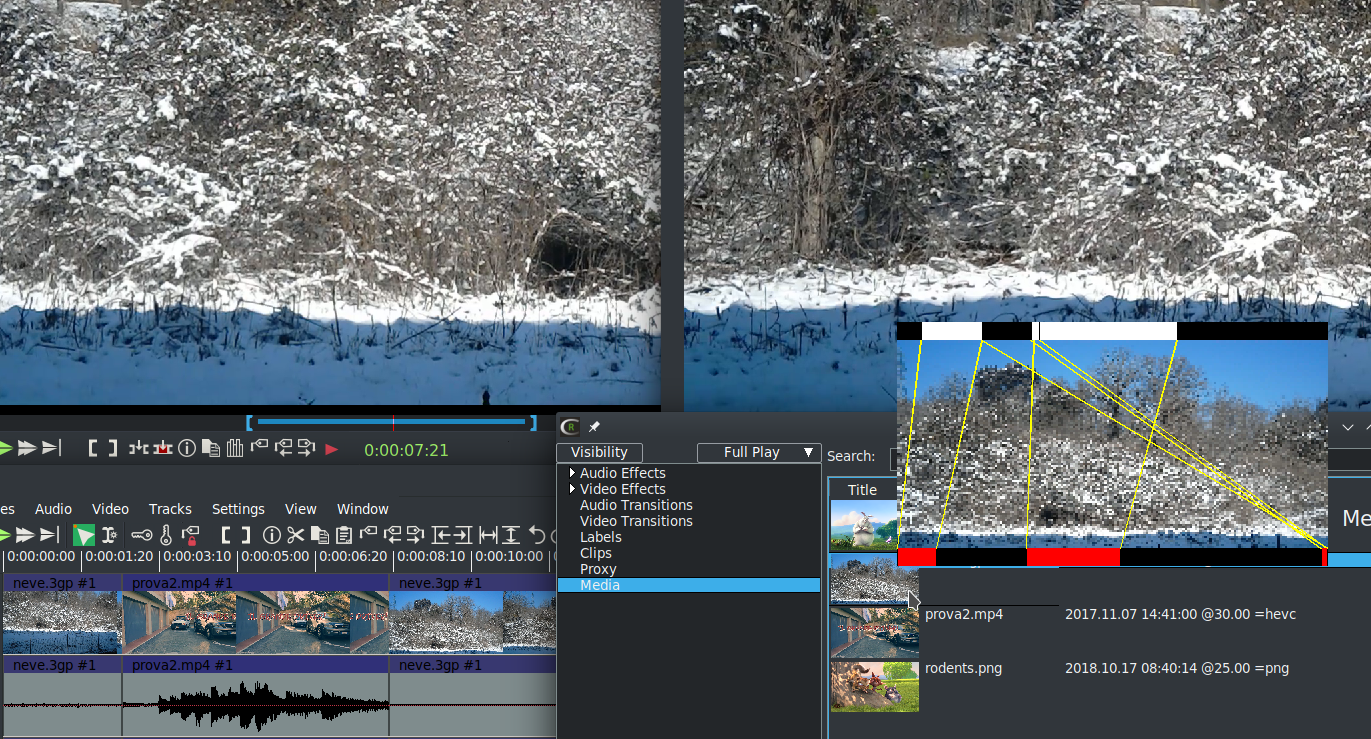
\includegraphics[width=1.0\linewidth]{inter-view02.png}
  \caption{Inter-View mode and the timeline}
  \label{fig:inter-view02}
\end{figure}

The Inter-View mode works for Media, Proxy, and User Bins.  When the
preview window has only black bars on the top and bottom, it means
that this particular media is not loaded in the timeline.  So when
you are in Proxy, meaning that the Proxy files are loaded on the
timeline, there will be only black bars for the corresponding Media
file UNLESS there is an audio track associated with the video.
Because audio tracks are not proxied, they will show for Media but
not for Proxy.


\section{Some Specific Editing Tools}%
\label{sec:specific_editing_tools}

This section covers some more detailed editing tools and scenarios
for edit management.

\subsection{Editing EDLs within a Project}%
\label{sub:edit-edls}

To edit EDL that is included with your project as Clips, Nested
Clips, Referenced File, or Xml you can use the option \textit{Open
  EDL} in the Resources window for the highlighted media.  Then with
a simple button click you can return to your main timeline project.
For example, if you have a nested clip that originally had several
plugins added to it before it was nested, you can edit those plugin
parameter values. Previously to make any changes to these types of
EDL you had to remake the whole clip from scratch.

Here is how this works. In the Clip or Media folder or on a timeline
EDL edit, the option \textit{Open EDL} for the highlighted clip or
nested clip is available so that when you choose this option, that
EDL will be brought up on the timeline superseding the current EDL
that exists on the timeline.  Now, once the clip is open on the
timeline, you can edit it however you want. The previous timeline
EDL is \textit{pushed onto a stack} so it can be recalled by
\textit{popping the stack} with a click of the left mouse button in
the upper right hand corner of the timeline to the left of the
\textit{shell cmds} icon.  Initially this button displays a 0 to
indicate your initial timeline/project.  Then this button will read
1 if you choose \textit{Open EDL} and then back to 0 and your
original timeline with the left mouse click.  You can go several
levels deep so instead of 1, it could be 2, 3, $\dots$ but this
requires some thought to avoid potential confusion.

An example of a typical set of steps to follow is:
\begin{enumerate}
\item Load your media using insertion strategy of \textit{Replace
    current project}.  There will be \# 0 in the upper right hand corner
  of the main menu with the tooltip of \textit{Close EDL}.
\item Highlight a selection on the timeline and press the
  \textit{To clip} icon and click the green checkmark OK.
\item In the Resources window, open the Clip folder and you will
  see that Clip 1 is present.
\item Highlight Clip1 and right mouse the item to bring up
  available options and select \textit{Open EDL}.
\item Now you will see the timeline change from the original
  media to just the clip content and the \# in the upper right hand
  corner will change from 0 to 1.
\item Add a visible effect, like AgingTV to the timeline.
\item Click on the \# 1 in the main menu bar to see he timeline
  restored to the original media.
\item Drag the clip from the Resources Clip folder to the
  timeline and you will see the AgingTV effect.
\end{enumerate}

You can follow the same steps as above by first using the option
\textit{Nest to media} in the Clip folder which nests the clip and
moves it out of the Clip folder to the Media folder.  Then use
\textit{Open EDL} on the Nested EDL in the media folder.  When you
Open EDL and edit the changes, those changes will take affect on any
and all occurrences of that nested clip on the current and/or
original timeline. The option to unnest that clip and put that back
into the Clip folder is the option \textit{EDL to clip}.  The nested
clip is still in the Media folder.  It will now have a name of the
next available Clip \# but the comment contains the previous name so
you can tell where it came from.

Instead of using the \# number on the main menu to close the current
EDL, both the Media and Clip folders have \textit{Close EDL} options
with the left mouse button. Clicking on the \# number is quick and
easy but for infrequent usage it is not obvious, whereas if you use
\textit{Open EDL} you see \textit{Close EDL} right below that and so
it is very obvious.  In addition in the case of where you have
opened a EDL, and you no longer see that clip in the folder, the
right mouse button where no media is highlighted will also display
the Close EDL option.

%\pagebreak
\begin{figure}[h]
  \centering
  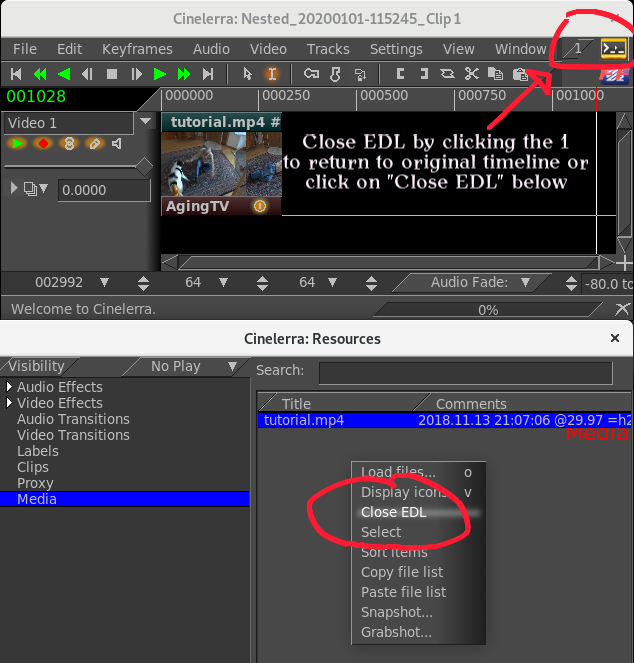
\includegraphics[width=1\linewidth]{editing-img001.png}
  \caption{Once you have an Open EDL, the easiest way to close it.}
  \label{fig:open_edl}
\end{figure}
\relax

In addition to the \textit{Open EDL} option in the Resources menu,
this option is available on the timeline when the cursor is on an
EDL-type edit. To get to this option, click on the middle mouse
button on that edit.  If it is not EDL, the option will not be
shown.  In summary:

\begin{center}
  \begin{tabular}{ll}
    \toprule
    Media folder of Resources window & Open EDL for Nested or Referenced EDLs\\
    Clip folder of Resources window & Open EDL for clips\\
    Track timeline & Open EDL for Nested or Referenced EDLs\\
    \bottomrule
  \end{tabular}
\end{center}

An aside -- when nesting and unnesting clips to take advantage of
this feature, names of the media can lead to some confusion.  For
example, if you nest a clip, the new name in the Media folder is the
word \textit{Nested} followed by an underscore with the date and
timestamp, another underscore, and then the clip name.  Then when
you unnest this Media folder clip via the \textit{EDL to clip}
option, the name will be changed in the Clip folder to the next
available Clip \#.  However the comment field will reflect the
nested clip name from which it was derived.  To avoid confusion you
can easily change the name for these clips in either the Clip or
Media folder because they are not real files at this point. To do
so, highlight the clip name in Resources, click on Info and type in
a new name.

For additional safety, the \textit{Open EDL} feature includes
additional backup capabilities. Automatically \CGG{} saves a backup
when certain changes are made or you can always use the shortcut `b'
to do one yourself, although keep in mind it will be overwritten
whenever \CGG{} wants to do another backup.  Now there is a shortcut
for the backup shortcut `b' so you can keep your hand on the mouse
instead of the keyboard.  Just click on the \# in the upper right
hand corner of the main window.  If \# is at 0, it backs up to
backup.xml, if at 1, it backs up to \texttt{backup1.xml} and so on
\dots up to \texttt{backup9.xml}.

When \textit{Open EDL} is invoked, the current EDL and current undo
stack are both \textit{pushed}, and the active session EDL is
replaced with the target clip/nested edl.  A new undo stack is
created, and the active \texttt{backup.xml} file name is decorated
with the stack level.  So, \texttt{backup.xml} is
\texttt{backup1.xml} when your edits are at stack level 1,
\texttt{back\-up2\-.xml} at stack level 2, and so on.  This means
that if you \textit{load backup} at stack level 1, the session will
reload from history at stack level 1, not the main session.


\subsection{Editing with File by Reference}%
\label{sub:file-reference}

It is sometimes handy to have EDL assets not as a copy, but as a
reference that is automatically updated into your project.  Suppose
you have several short videos that at the end have the same credits
which include the current year such as 2019.  But now it is 2020 and
all of the videos would have to be individually updated with the new
date.  By including a \textit{Referenced File} as the EDL file type
when you create each of the videos, you can just change the one
credits xml file and the next time you load one of the videos and
render it, it will now automatically have the updated information.

The purpose of this feature is to be able to rework a smaller
section of a global master project at any time, which can be done by
an "assistant" and then this work is automatically reflected in the
global master project.  It is for \textbf{advanced usage only}.

Up until the addition of this feature, \CGG{} has always used copies
and no direct reference in order to ensure original data is never
compromised.  In the usual case, subprojects as xmls are copied into
a master project where subprojects had been inserted, so that if you
change something in a subproject or delete a subproject, it would
have no affect on the master project.  But now with \textit{File by
  Reference}, any project that uses a referenced file will
automatically include any changes made to the referenced file when
loaded.  At the same time, if you use the EDL file NOT as a
referenced file in a project since it is then just a copy, it will
not be updated.  Because of this difference, the user needs to be
very aware of what using this feature could do.

\textbf{Use with extreme caution}.  However, there are several
built-in safety features and a warning that should never be turned
off even though it gives you the option to do so.  These include:

\begin{enumerate}
\item When the \texttt{File, Load files} menu is opened, the EDL
  strategy will always be set to just EDL as default.  Although, if
  you use Apply and leave the Load Menu open, it will stay changed to
  what you selected until it is re-opened.
\item When an EDL is opened as \textit{Reference}, the color of
  that file name in the Resources Media folder is different in order
  to serve as a reminder that it is special.
\item A warning message is displayed in a popup window when you
  load a \textit{File by Reference} that reads “Other projects can
  change this project and this can become a broken link”.  Although
  you can check the warning box to never see this warning again, you
  would be well advised to not do so.  It is a great reminder of
  consequences and you will not want to be cavalier about the warning.
  Instead just use the X to dismiss the warning.
\end{enumerate}

Here is a step by step example of how you can use \textit{File by
  Reference}:
\begin{enumerate}
\item Start up \CGG{} and use the Title plugin to create a new
  credits file.  Save as credits.xml.
\item Start a New project and then load an existing master
  project to the timeline.
\item Load the credits file you created in step 1 with a Load
  Strategy of Create Resources Only and with EDL Strategy as
  \textit{Reference}.
\item Note the color change in the credits.xml filename and the
  reference comment in the Resources Media folder.
\item Drag the credits file to an empty spot on the timeline.
  Save this new master project and quit.
\item Start \CGG{} up again.  Load credits.xml and make a change
  to the Title and save again.
\item Exit \CGG{}; restart \CGG{}; load your master project and
  now you will automatically see on the timeline the changes you just
  made in the previous step.
\end{enumerate}


\subsection{Edit Length}%
\label{sub:edit-lenght}

To set the length of an edit in the timeline, select the region
which contains the edit to be modified. Now select the menu bar
\texttt{Edit $\rightarrow$ Edit Length}\dots menu item to activate
the \textit{edit length} popup (figure~\ref{fig:lenght}).  The
duration of the edit can be reset by entering the desired edit
length in seconds.  Pressing OK will change all of the selected
edits (in armed tracks) to the specified length.

\begin{figure}[htpb]
    \centering
    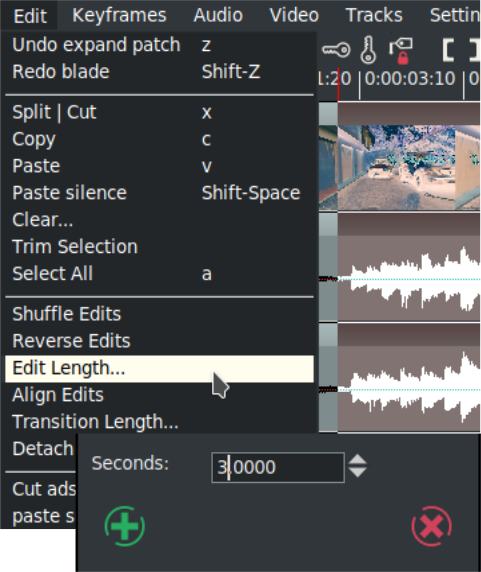
\includegraphics[width=0.5\linewidth]{lenght.png}
    \caption{Edit Length window}
    \label{fig:lenght}
\end{figure}

\subsection{Align Edits}%
\label{sub:align_edits}

When loading media, a common problem is that the various audio/video
tracks do not always have exactly the same lengths. For example, you
might load audio/video recordings from your camera and be dismayed
to see that the audio for each segment is a half second longer than
the video. If you load a large set of media clips by concatenation,
the audio and video will be more skewed as more media is
loaded. Align Edits makes it possible to adjust the edits so the
audio and/or video align by adjusting
the edits so that the track lengths are consistent. To use this
feature, load all of the desired media and select a region which
contains all of the edits to be aligned in the timeline. Now select
the menu bar \texttt{Edit $\rightarrow$ Align Edits} menu item to
operate the change. The topmost armed track is used as a template
reference, and the rest of the tracks are either cut or padded to
align the edit boundaries.  Besides aligning audio with the video,
you can also align video with the audio if the first armed track is
audio. The code performs the following algorithm:

\begin{itemize}
\item Use the first armed track as the master track (it must
  contain data).
\item Collect the \textit{edit project start times} on the
  selected master track. Only edits that are 100\% inside the selected
  area will be used.
\item Set all other tracks to match the \textit{edit times} of
  the template track, either by putting in silence or cutting the
  region to align the edits on the \textit{edit times} of the master
  track.
\end{itemize}

The start time sequence of media and silence edits
along the master track are collected as the target alignment
boundaries. All armed tracks after the master track are modified so
that if the next edit edge is too soon, it adds silence; if it is
too late, edits are shortened or deleted past the point of the next
target alignment boundary time.  Align Edits works best if there are
an equal number of Video and Audio sections.  Also, it is better to
use cuts instead of adding silence -- if there are silence edits
together, the algorithm will combine the silence edits into a single
edit and results may not be as desired.

The first two screenshots in figure~\ref{fig:align} show the Before,
the Highlighted Edits to be manipulated, and the After results for
the Align Edits. The third screenshot \textit{adds silence} in the
second section as noted in red letters.

\begin{figure}[htpb] \centering
  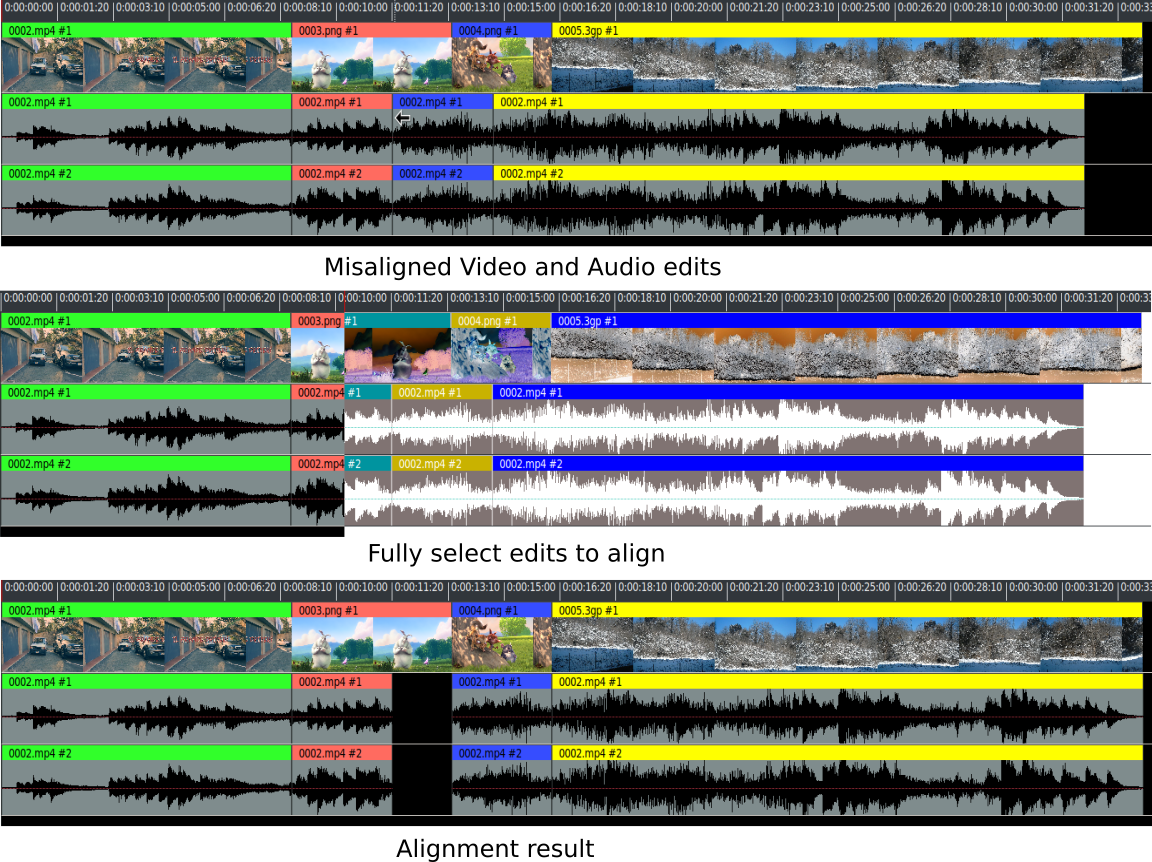
\includegraphics[width=1.0\linewidth]{align.png}
  \caption{Align edits}
  \label{fig:align}
\end{figure}


\subsection{Reverse Edits}%
\label{sub:reverse_edits}

The Reverse Edits can be useful to change the order of 2 edits in
the case where you would like to put a \textit{teaser} section that
occurred in the middle of a movie at the beginning instead, that is,
reversed positions.  To operate, highlight completely the edit areas
you would like reversed and then use the pulldown \texttt{Edit
  $\rightarrow$ Reverse Edits}.

Figure~\ref{fig:reverse01} shows the selected / highlighted area to
which Edits will be applied.  Note the first edit is 0002, followed
by 0003, 0004, and 0005 in that order.

\begin{figure}[htpb]
  \centering
  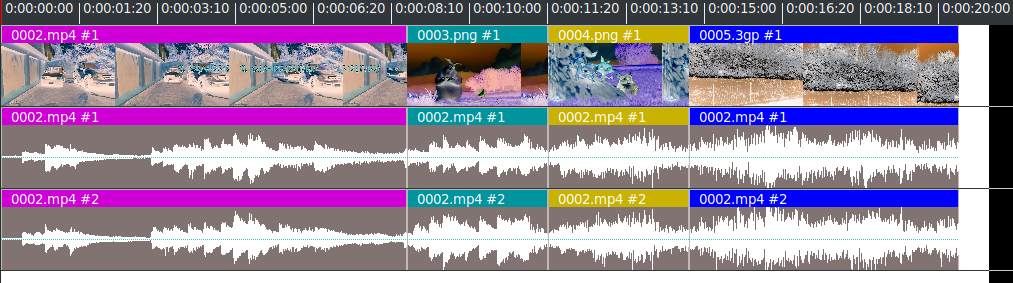
\includegraphics[width=0.9\linewidth]{reverse01.png}
  \caption{Selected area for Reverse Edits}
  \label{fig:reverse01}
\end{figure}

Figure~\ref{fig:reverse02} shows the results of executing
\textit{Reverse Edits}.  Now you will see the reversed order of
0005, 0004, 0003, and last 0002.

\begin{figure}[htpb]
  \centering
  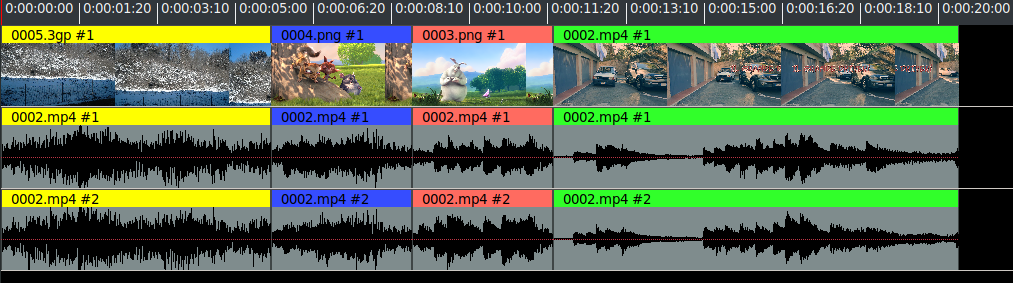
\includegraphics[width=0.9\linewidth]{reverse02.png}
  \caption{Results of the Reverse Edits}
  \label{fig:reverse02}
\end{figure}


\subsection{Shuffle Edits}%
\label{sub:shuffle_edits}

The file pulldown \texttt{Edit $\rightarrow$ Shuffle Edits} will
randomly exchange the location of the edits.  This feature can be
used to change the order of the music like you would do from your
MP4 player where you have a playlist of your favorite music.  Or
perhaps you are creating an advertisement background, you can
randomly change it, thus the viewer sees a different order of scenes
each time shown.

Figure~\ref{fig:shuffle} illustrating Shuffle Edits of the
highlighted area of the first screenshot on the page.  Note the
permutation of the fragments resulting in 0002 now being first, then
0004, 0003, and 0005 last.

\begin{figure}[htpb]
  \centering
  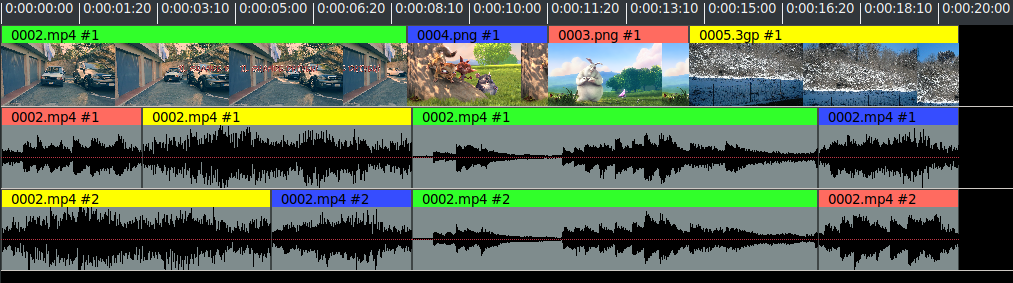
\includegraphics[width=0.9\linewidth]{shuffle.png}
  \caption{Shuffle edits: the edits are permutated}
  \label{fig:shuffle}
\end{figure}


\subsection{Drag Handle Management / Trimming}%
\label{sub:drag_handle_management_trimming}

With some edits on the timeline it is possible to do trimming. By
trimming you shrink or grow the edit boundaries by dragging them. In
drag and drop mode or cut and paste mode, move the cursor over an
edit boundary until it changes shape. The drag handle shows as a
left or right facing fat arrow when you cursor near the clip start
or end.  If the cursor faces left, the dragging operation affects
the beginning of the edit. If the cursor faces right, the dragging
operation affects the end of the edit.

The effect of each drag operation not only depends on the behavior
button but whether the beginning or end of the edit is being
dragged. When you release the mouse button, the trimming operation
is performed.

For all file formats, other than still images, the extent of the
trimming operation is limited to the source file length. Attempting
to drag the start of the edit beyond the start of the source, limits
it to the source start. In all trimming operations, all edits which
start on the same position as the cursor when the drag operation
begins are affected. You have to disarm tracks in order to prevent
edits from being affected.

You have 6 different choices of which mouse button to use for
specific types of editing while using the drag handle.  You change
the drag handle mouse effects by using the \texttt{Settings
  $\rightarrow$ Preferences  $\rightarrow$ Interface} tab and
modifying the Editing section as shown in the next
figure~\ref{fig:trim}. The drag handle affects not only the clip you
are working on but also frequently the entire duration of all clips
on the timeline.

\begin{figure}[htpb]
  \centering
  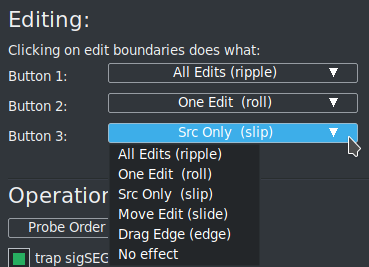
\includegraphics[width=0.6\linewidth]{trim.png}
  \caption{Default choices for mouse: Ripple for button 1; Roll
    for button 2; Slip for button 3}
  \label{fig:trim}
\end{figure}

A description of the fundamental/common terminology for choices
follows.

\begin{description}
\item[All Edits (ripple)] shorten or lengthen the start or end
  of a single piece of media while moving all media to the right of
  that clip up or down on the timeline correspondingly.  Timeline
  duration is modified.  In a drag \textit{All Edits} operation, the
  beginning of the edit either cuts data from the edit if you move it
  forward or pastes new data from before the edit if you move it
  backward. The end of the edit pastes data into the edit if you move
  it forward or cuts data from the end of the edit if you move it
  backward. All the following edits shift. If you drag the end of the
  edit past the start of the edit, the edit is deleted.
\item[One Edit (roll)] move the in and out point of a single
  clip without changing the timeline duration. In a drag \textit{One
    Edit} operation, nothing is cut or pasted. If you move the beginning
  or end of the edit forward, the source reference in the edit shifts
  forward. If you move the beginning or end of the edit backward, the
  source reference shifts backward. The edit remains in the same spot
  in the timeline but the source shifts.
\item[Src Only (slip)] move the in and out point of a single
  clip without changing the timeline duration. In a drag \textit{Src
    Only} operation, nothing is cut or pasted. If you move the beginning
  or end of the edit forward, the source reference in the edit shifts
  forward. If you move the beginning or end of the edit backward, the
  source reference shifts backward. The edit remains in the same spot
  in the timeline but the source shifts.
\item[Slide] a single clip is moved but retains its current in
  and out point; however the out point of the clip to the left changes
  and the in point of the clip to the right also changes.  Timeline
  duration remains the same.
\item[Edge Left/Right] moves the edge of the clips.
\item[No effect] no changes are made.  You might want to use
  this choice to prevent accidental movements.
\end{description}

The next table displays the options and results
with the Key Table here first.

\begin{lstlisting}[style=sh]
    s = src media start
    p = proj position
    l = length
    c = cut distance
    rest == p+=c: for rest of clips
    01 = flags edits_moved, rest_moved
\end{lstlisting}

\renewcommand{\arraystretch}{1.15}
\begin{table}[ht]
  %\caption{}
  %\label{tab:}
  % Tell table to adjust font to fix on the page using \resize
  \resizebox{\textwidth}{!}{%
    \begin{tabular}{lllll}
      \toprule
      &  & \textbf{Drag Left} & \textbf{Drag Right} &\\
      \midrule
      \multicolumn{2}{l}{\textit{curr s += c, l -= c; + rest}} & $\leftarrow$ & $\rightarrow$ & \textit{rest}\\
      abc12345xyz & \textbf{Ripple} left edge 11 $\rightarrow$ & abc012345xyz & abc2345xyz &\\
      \midrule
      \multicolumn{2}{l}{\textit{curr l += c; + rest}} & $\leftarrow$ & $\rightarrow$ & \textit{rest}\\
      abc12345xyz & \textbf{Ripple} right edge 01 $\rightarrow$ & abc1234xyz & abc123456xyz &\\
      \midrule
      \multicolumn{2}{l}{\textit{prev l += c; curr ps+= c, l -= c}} & $\leftarrow$ & $\rightarrow$ &\\
      abc12345xyz & \textbf{Roll} left edge 00 $\rightarrow$ & ab012345xyz & abcd2345xyz &\\
      \midrule
      \multicolumn{2}{l}{\textit{curr l += c; next ps+= c, l -= c}} & $\leftarrow$ & $\rightarrow$ &\\
      abc12345xyz & \textbf{Roll} right edge 00 $\rightarrow$ & abc1234wxyz & abc123456yz &\\
      \midrule
      \multicolumn{2}{l}{\textit{s -= c}} & $\leftarrow$ & $\rightarrow$ &\\
      abc12345xyz & \textbf{Slip} left edge 10 $\rightarrow$ & abc23456xyz & abc01234xyz &\\
      \midrule
      \multicolumn{2}{l}{\textit{s -= c}} & $\leftarrow$ & $\rightarrow$ &\\
      abc12345xyz & \textbf{Slip} right edge 10 $\rightarrow$ & abc23456xyz & abc01234xyz &\\
      \midrule
      \multicolumn{2}{l}{\textit{prev l += c; curr p+= c; next ps += c, l -= c}} & $\leftarrow$ & $\rightarrow$ &\\
      abc12345xyz & \textbf{Slide} left edge 10 $\rightarrow$ & ab012345wxyz & abcd12345yz &\\
      \midrule
      \multicolumn{2}{l}{\textit{prev l += c; curr p+= c; next ps += c, l -= c}} & $\leftarrow$ & $\rightarrow$ &\\
      abc12345xyz & \textbf{Slide} right edge 10 $\rightarrow$ & ab12345wxyz & abcd12345yz &\\
      \midrule
      \multicolumn{2}{l}{\textit{curr s -+= c, l += c; + rest}} & $\leftarrow$ & $\rightarrow$ & \textit{rest}\\
      abc12345xyz & \textbf{Edge} left edge 11 $\rightarrow$ & abc2345xyz & abc0123456xyz &\\
      \midrule
      \multicolumn{2}{l}{\textit{curr l -+= c; + rest}} & $\leftarrow$ & $\rightarrow$ & \textit{rest}\\
      abc12345xyz & \textbf{Edge} right edge 01 $\rightarrow$ & abc1234xyz & abc123456xyz &\\
      \bottomrule
    \end{tabular}
  }
\end{table}
\renewcommand{\arraystretch}{1}

Next, a more immediate and colorful view shows these trimming
options (figure~\ref{fig:trim-color}).

\begin{figure}[htpb]
    \centering
    \includegraphics[width=0.8\linewidth]{trim-color.png}
    \caption{The 5 types of Trim: note the different lengths of the results.}
    \label{fig:trim-color}
\end{figure}

\paragraph{How to do a J-cut or L-cut} A J-cut is a split edit film
editing technique in which the audio from a following scene overlaps
the picture from the preceding scene, so that the audio portion of
the later scene starts playing before its picture as a lead-in to
the visual cut.  An L-cut is a different split edit film editing
technique in which the audio from preceding scene overlaps the
picture from the following scene, so that the audio cuts after the
picture, and continues playing over the beginning of the next scene
(figure~\ref{fig:j-cut}). To do either a J-cut or an L-cut, you
first shorten the first or second video a little.  Then you block
the audio tracks from changing by disarming the appropriate tracks.
Finally use \textit{One Edit (roll)} the cutting edge off the
videos.  Moving to the right creates a J-cut and moving to the left
creates an L-cut.

\begin{figure}[htpb]
    \centering
    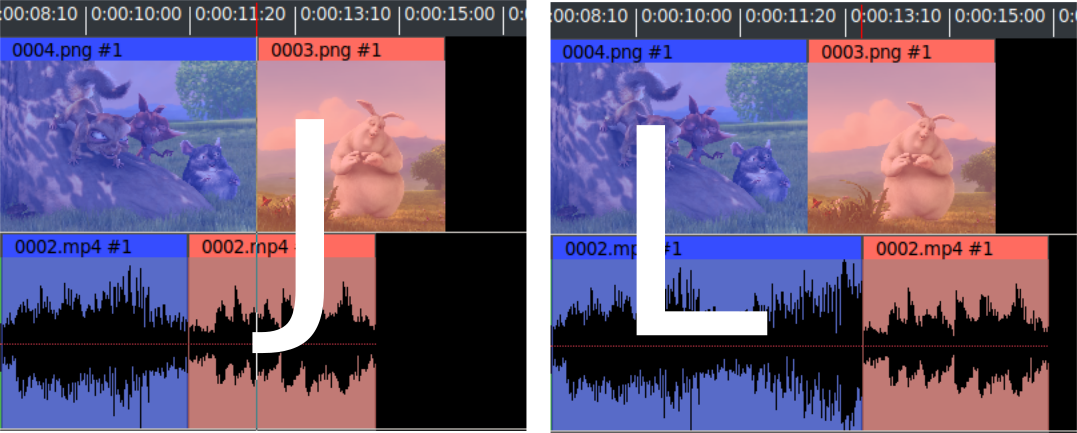
\includegraphics[width=0.8\linewidth]{j-cut.png}
    \caption{J-cut to left and L-cut to right}
    \label{fig:j-cut}
\end{figure}


\subsection{Split View in Compositor Using the Drag Handle with Trim}%
\label{sub:split_view_compositor_using_drag_trim}

The Trim Feature using the drag handle provides some good ways to
view your video while editing.  The playback position in the
compositor is updated live and the view in the compositor can be
split so that in the left half of the compositor you can see the
last frame of the left clip and in the right half the first frame of
the right clip.  Dragging edits can not be extended past the
beginning or the end.

First familiarize yourself with button operation; check your setup
by executing the following step.  In the \texttt{Settings
  $\rightarrow$ Preferences $\rightarrow$ Interface} tab, Editing
section, clicking on the edit boundaries can be set for Button 1, 2,
3 as one of the following:

\textit{Ripple}; \textit{Roll}; \textit{Slip}; \textit{Slide};
\textit{Edge} or \textit{No effect}

Now to use this feature, create a track with edits that have trims
on the left and/or the right. The edit boundary can be modified
using \textit{drag handles} at the boundary between the edits
(figure~\ref{fig:trim-display}).

\begin{figure}[htpb]
  \centering
  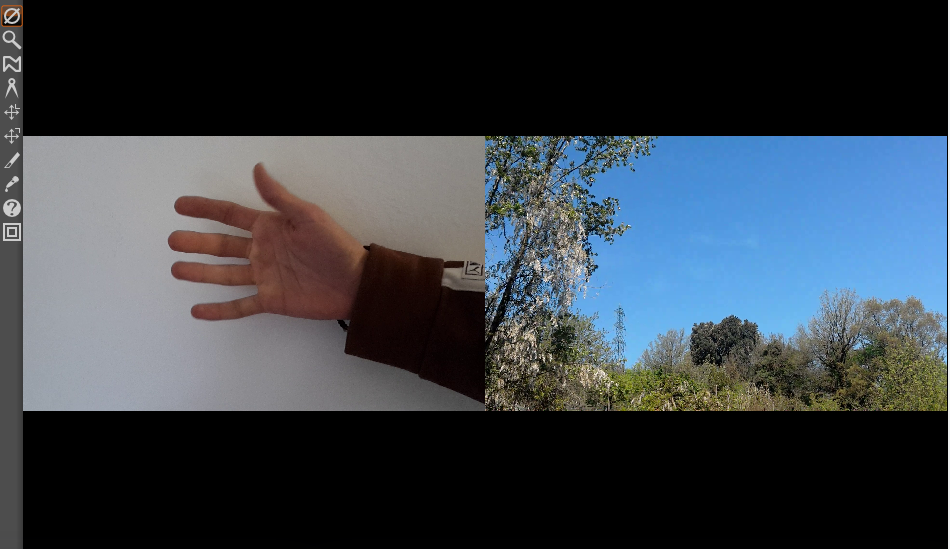
\includegraphics[width=1\linewidth]{trim-display.png}
  \caption{Split compositor screen showing the result of the Trim feature}
  \label{fig:trim-display}
\end{figure}

\begin{description}
\item[Left Mouse Button (LMB) usage:] If you grab the edit
  handle from the right side, you will see a left arrow and dragging
  the boundary will modify the right edit playback starting time. If
  you grab the edit handle from the left side, you will see a right
  arrow and dragging the boundary will modify the left edit playback
  ending time. In both cases, the composer will show the edit endpoint
  of the changed edit.
\item[Shift LMB usage:] The effect on the edits is the same as
  described above, but the composer will show a split screen of the
  left and right edits as they appear at the drag handle
  boundary. Dragging will only change one of the two images, since
  only one edit is being changed.
\item[Middle Mouse Button (MMB) usage:] Both the left and the
  right edit ending/starting times are updated.  The image shown in
  the compositor will be drawn from the side of the drag grab, that is
  the left if it is grabbed from the left, and the right if it is
  grabbed from the right.
\item[Shift MMB usage:] The effect on the edits is the same as
  described above, but the composer will show a split screen of the
  left and right edits as they appear at the drag handle boundary.
  Dragging will change both of the two images, since both edits are
  being changed.
\item[Right Mouse Button (RMB) usage:] The start/end point of
  the current edit is moved, but the edit length is unchanged only one
  image changes since only one edit endpoint is view is updated.
\item[Shift RMB usage:] The effect on the edits is the same as
  described above, but the composer will show a split screen of the
  left and right edits as they appear at the drag handle boundary.
  Dragging will only change one of the two images, since only one edit
  is being changed.
\end{description}


\subsection{Snapping while Cutting and Dragging}%
\label{sub:snapping_cutting_dragging}

\paragraph{Cutting/Snapping edits} cuts from an edit handle to the
insert point.  There are Edit Panel buttons which normally are used
to move to the previous or next edit handle/label.

\begin{wrapfigure}[3]{r}{0.2\linewidth}
  \vspace{-2ex}
  \centering
  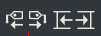
\includegraphics[width=0.7\linewidth]{snap.png}
\end{wrapfigure}

They look like tags and the letter E on the menu bar and are
oriented forward/backward.  These same buttons can be used to
\textit{cut} from the insert pointer to the previous or next
edit/label when the ctrl+alt keys are both pressed when the buttons
are used.  They \textit{snap} off the media instead of doing the
standard re-positioning.  This is useful to minimize the number of
operations necessary to cut between edits/labels.

Instead of using the edit panel buttons, you can more easily use the
following keyboard shortcuts to perform the same functions:

\begin{center}
  \begin{tabular}{lll}
    \toprule
    snap\_right\_edit & ctrl+alt+ '.' &\\
        snap\_left\_edit & ctrl+alt+ ',' &\\
    snap\_right\_label & ctrl+alt +shift '.' & shift+period is the > sign on US keyboards\\
    snap\_left\_label &  ctrl+alt +shift',' & shift+comma is the < sign on US keyboards\\
    \bottomrule
  \end{tabular}
\end{center}

\paragraph{Drag Snapping} if you hold down the Ctrl + Alt keys while
dragging using the mouse, once the clip gets near to an edit, a
label, an in/out pointer or the start/end of the timeline, the
dragged clip will snap next to that marker.  The 2 will now be
exactly aligned with no gap and no overlap.  As you drag the clip
close to one of the markers, when they are within a short distance
they start to stick and stay that way until you move further away
from that distance.  Also, the line will turn color from green to
yellow while in the sticky phase.


\subsection{Nesting}%
\label{sub:nesting}

\paragraph{Nested Assets} A nested asset is an EDL session that
embeds an existing EDL session, all tracks, all plugins, editing,
and effects into a media object that appears as one audio/video
media object, no plugins, editing, or effects.  It is as if the
existing EDL was rendered, and loaded in its place.  This has
several interesting side effects.  First, you don’t have to render
the entire media file to see any portion.  Second, it requires no
rendering compute time or storage.  Third, it changes the precedence
of the composer so that you get more control over the projection and
automation, so that the results can be sent into another rendering
step, not simply part of the current stack.  It groups the plugin
stack in much the same way that an arithmetic expression is grouped
by parenthesis.

The EDL session and the rendered output are visually equivalent.
Nested assets allow for complex grouping and stacking of effects,
and makes media access much more flexible.  This feature can be used
recursively, that is, any number of sessions may be stacked and
referenced as an asset, as long as all of the rendering resources
are available.  Nested assets are added to the timeline by using the
pulldown \texttt{File $\rightarrow$ Load files}\dots on the main
menu and selecting the \textit{Insertion strategy} of \textit{Nest
  asset}. The file will be pasted into the timeline over the current
selection or at the insertion point.

It is somewhat important to note that nested assets and nested clips
will have index files automatically created.  These index files can
start to clutter up your \texttt{\$HOME/.bcast5} directory with
files named \texttt{Nested\_\#\#\#.idx} and you may want to
periodically delete any index files which are no longer in use.

\paragraph{Nested Clips} It is also possible to create
\textit{clips} and convert them to \textit{nested edl}.  This is
done by first creating a clip using the standard cut, clipboard,
paste, and/or edit panel buttons.  Now, using the resources
\textit{clip} folder, select a clip to be nested, and use the right
mouse button to select a clip.  This activates the clip popup menu.
Select the \textit{Nest to media} menu item, and the clip will be
converted to a \textit{Nested: Clip} and put in Media
folder. Conversely, you can select a \textit{Nested: Clip}, use the
\textit{EDL to clip} menu item, and the clip will be reverted to a
\textit{Clip}.  This works similarly to the group / un-group editing
features of many graphic design editing programs, but in this case
the groups are rendered compositions (figure~\ref{fig:nesting}).

Nested clips can be proxied and when they are, the resulting files
are placed in the user's \$HOME/Videos directory by default.  This
can be modified by changing

\texttt{Settings $\rightarrow$ Preferences $\rightarrow$ Interface}
tab, Nested Proxy Path.

\begin{figure}[htpb]
  \centering
  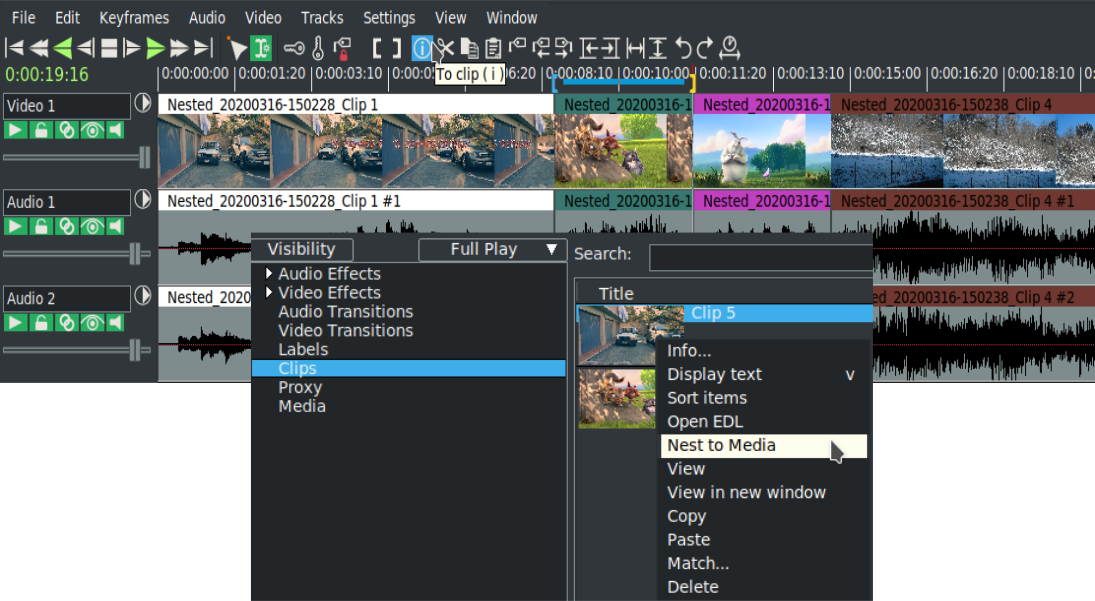
\includegraphics[width=1.0\linewidth]{nesting.png}
  \caption{Nested clips in Timeline and Resources window}
  \label{fig:nesting}
\end{figure}

\paragraph{Usage Examples of Nested Clips}

\begin{description}
\item[Example 1:] You want to make a flashback/rewind at the end
  of your video that represents a quick summary of the entire video in
  black and white. On he timeline, you have 60 seconds of edits with
  clips, cuts, zoom in, zoom out and any other edits. Now you want to
  get this 60 seconds \textit{compressed} to 10 seconds, play in
  reverse, and in black and white at the end of your video.  You would
  copy the 60 seconds in a clip, nest the clip in the Clip folder of
  the Resources window and drag it to the timeline. You will see only
  a clean clip without all of the edits that were used to create it
  because nesting display a clip without having to actually use the
  Render menu.  Now you can add a Reverse effect, Color3way plugin for
  black and white, and use the Speed auto to get the 60 seconds down
  to only 10 seconds.
\item[Example 2:] You are working on a complex project with a
  team in a separate location. You create some sub projects, i.e.\
  sequences, that you or the team will use in the Master project to
  merge the sequences in the right order and to make the final color
  correction steps.
\end{description}

In each of the examples you can see the benefit of nesting to create
clean looking timelines because of the automatic rendering
capability of nesting.


\subsection{Copy/Paste clips/medias across Multiple Instances}%
\label{sub:copy_paste_multiple_instances}

It is easy to copy/paste clips/media within a single instance of
\CGG{} or across multiple instances.  The reason this works is
because there are hidden X cut buffers and these are used to
transmit EDL from 1 instance to another.

Steps to copy from a source timeline and paste to a target timeline:

\begin{enumerate}
\item highlight a selection on the timeline in 1 instance of \CGG{}
\item use the Copy icon (shortcut c) on the main menu bar to copy
  into a buffer
\item move the pointer to another instance of \CGG{} and set an
  insertion point in its timeline
\item use the Paste icon (shortcut v) to paste the clip to that
  other instance selection target
\end{enumerate}


\section[ShuttlePROv2 and ShuttleXpress Jog Wheels for Editing]{ShuttlePROv2 and ShuttleXpress Jog Wheels for Editing\protect\footnote{programmatic specifications from Eric Messick}}%
\label{sec:shuttle_jog_wheels_editing}

The ShuttlePROv2 and ShuttleXpress are affordable jog wheels which
can be useful for working with Cin, especially if you do a lot of
playing forward/backward, fast/slow/normal, and single frames
(figure~\ref{fig:shuttle}).
%
Directions for using the ShuttlePROv2 and the ShuttleXpress with
\CGG{} are described next. These devices work by sending keystrokes
used in Cin, corresponding to the shuttle action, to the keyboard
buffer. The shuttle has been fully integrated into the \CGG{} code
so that after the one initial setup, no further intervention is
required.  The multi-speed outer wheel works the same and has the
same number of S positions on both shuttles but the shuttle Xpress
has only 5 keys.  Since the majority of user operations will most
likely be with the use of the 2 wheels, the slightly smaller Xpress
could be a better choice with its 5 easy to reach keys.  The Pro is
approximately $4\times7$\,inches whereas the Xpress is about
$4\times4$\,inches.

\begin{figure}[htpb]
  \centering
  \includegraphics[width=0.9\linewidth]{shuttle.png}
  \caption{ShuttlePROv2 and ShuttleXpress}
  \label{fig:shuttle}
\end{figure}

The vendor supplied \textit{string} device names for the shuttles
are currently:

\texttt{/dev/input/by-id/usb-Contour\_Design\_ShuttlePRO\_v2-event-if00}\\
\texttt{/dev/input/by-id/usb-Contour\_Design\_ShuttleXpress-event-if00}\\
\texttt{/dev/input/by-id/usb-Contour\_Design\_ShuttlePro-event-if00}

Only 1 necessary initial setup is required due to permission
settings for non-root usage. As root, just copy a file that provides
the necessary permissions to use the shuttle, then reboot, Example
copy:

\begin{lstlisting}[style=sh]
sudo cp {cindat_path}/doc/99-ShuttlePRO.rules /etc/udev/rules.d/
\end{lstlisting}

then the next time after you reboot, the permissions should be
correct. This file only needs to contain one of the following lines
depending on which shuttle version you have/use, but all will be in
the file.

\begin{lstlisting}[style=sh]
# for  newer PRO model
ATTRS{name}=="Contour Design ShuttlePro" MODE="0644"
# for older PRO model
ATTRS{name}=="Contour Design ShuttlePRO v2" MODE="0644"
# for the Xpress model
ATTRS{name}=="Contour Design ShuttleXpress" MODE="0644"
SUBSYSTEMS=="usb", ATTRS{idVendor}=="0b33", ATTRS{idProduct}=="0020", MODE="0666"
SUBSYSTEMS=="usb", ATTRS{idVendor}=="0b33", ATTRS{idProduct}=="0030", MODE="0666"
\end{lstlisting}

If you swap your shuttle, for example upgrade from an Xpress to a
PROv2, just stop Cin, unplug the original shuttle, plug in the
replacement shuttle, and restart Cin.  If you start the \CGG{}
program and the shuttle does not function as before, stop \CGG{} and
then simply unplug it and plug it in again.  There are a couple of
reasons why it may stop functioning.  One is because \CGG{} was not
stopped with the usual Quit command and the shuttle was improperly
shut down when there was a crash.  The other possibility is that a
static discharge occurred in the area.

A default shuttlerc file is automatically used when a shuttle device
is plugged in when Cin is started. This file sets up the key
bindings for \CGG{} to use. You can override any default settings by
having a local file in your \texttt{\$HOME} directory, named
\texttt{.shuttlerc} to reflect your personal preferences.


\subsection{How to Modify the Default Key Settings}%
\label{sub:modify_default_key_settings}

Detailed information on how to modify your local \texttt{.shuttlerc}
file is described next, but if you need help you can request more
information in the forum at {\small
  \url{https://cinelerra-gg.org}}. In the \texttt{shuttlerc} file, a
\# always represents a comment and blank lines are ignored.  The
first thing you must do is copy the system supplied
\texttt{shuttlerc} file to your \texttt{\$HOME} directory and rename
it as \texttt{.shuttlerc} (with a period).

The \texttt{shuttlerc} file has sections that in the case of \CGG{},
represent different windows allowing you to set the keys, K1-K15 for
the Pro and K5-K9 for the Xpress, the shuttle wheel positions of
S0/S1/S-1 for stop, S2 through S7 for wheeling to the right, and S-7
through S-2 for wheeling to the left for reverse.  Then there is JR
to jog right (clockwise) and JL to jog left (counter-clockwise) for
the inner smaller wheel for single frame movement.  See the key
arrangement on a later page for location of the keys for each of the
two different shuttles.

The sections are surrounded by brackets for windows such as \CGG{}
(the main window), Viewer, Composer, Resources, Load, and Default.
If you want the keys to be defined the same in every window, you can
bracket each window on lines one right after the other and then just
define one set of keys.  The other lines will have the key
name/shuttle position followed by its assigned value.  The values
you use for the keys are usually shortcuts and have to be
operationally defined within \CGG{}. For example, the shortcut “f”
to go fullscreen is defined so can be used; however the shortcut “h”
is not defined so will not do anything.  You can check the file,
shortcuts.html, for some options to use.

Next are a few actual examples from the default
\texttt{{cindat\_path}/shuttlerc} file.

The next brackets represent sections. Default, Resources, Load
windows all use the same key values.

\begin{lstlisting}[style=sh]
[Default]
[Resources]
[Load]
K5 XK_Home
K6 XK_Button_1 # same as mouse button 1
K7 XK_Button_2 # same operation as mouse button 2
K8 XK_Button_3
K9 XK_End
# for example, in the Load menu, use scroll up to get to the next file name
JL XK_Scroll_Up
JR XK_Scroll_Down
\end{lstlisting}

Cinelerra with brackets around it next, is the section with some key
definitions for the main window.

\begin{lstlisting}[style=sh]
[Cinelerra]

# Most useful functions have to be on K5-K9
# because Xpress only has 5 keys
K5 XK_Home      # Beginning
K6 XK_KP_6      # Reverse, or if playing Stop
K7 XK_KP_0      # Stop
K8 XK_KP_3      # Play, or if playing Stop
K9 XK_End       # End
...
S-7 REV_16     	# Next 6 are reverse keys
S-6 REV_8      	#  the number on the end represents speed
S-5 REV_4      	#  number can be decimal up to 64
S-4 REV_2      	#  2 means 2x or double speed
S-3 REV_1
S-2 REV_0.5    	#  0.5 represents 1/2 speed
S-1 XK_KP_0    	# Because the Shuttle does not generate S0,
		#   have to use S-1
S0  XK_KP_0   	# Hardware does not generate S0
S1  XK_KP_0   	# Because the Shuttle does not generate S0,
		#   have to use S1
S2  FWD_0.5
S3  FWD_1
...
\end{lstlisting}

An explanation for the above REV and FWD key symbol values is
necessary to facilitate user preferences.  Obviously REV stands for
reverse and FWD for forward.  You can set any speed up to and
including 64x (that is, 64 times the normal speed) on any of the S
keys.  First in the line is the key name such as S-3 and then the
key direction of FWD or REV followed by the symbol for underscore
(\_) and then the numerical value to use.  For example, if you want
the $5^{th}$ forward position, S5, to play 10$\frac{1}{2}$ times
faster, you would use the statement \texttt{S5 FWD\_10.5}.  Integer
or decimal numbers are legal.

For the Viewer, you may want keys defined to do a Splice or an
Overwrite so define differently.  Note that assignments that contain
single character letters must be enclosed in quotes.

\begin{lstlisting}[style=sh]
[Viewer]
# Splice - Viewer only; may be defined
# differently than Composer or Cinelerra
K2 "v"
K4 "b"		# Overwrite
\end{lstlisting}

To change any key value to an alternative value, just edit the file
and make the changes.  Besides just keys and alphabetic letters of
numbers, you can also use any \CGG{} value that contains the
combination with Shift, Alt, and Ctrl.  For keys that are not
printable characters, you can look up the symbol name to use for a
specific operation in the file called:
\texttt{/usr/include/X11/keysymdef.h}. Some examples:

\begin{lstlisting}[style=sh]
K10 Alt-XK_Left	  # Go to previous edit \\
K13 Ctrl-XK_Right # Go to next label
\end{lstlisting}

For sequences of one or more \textit{printable} characters, you can
just enclose them in double quotes.  For example in the
\texttt{[Composer]} section, to go into or out of fullscreen mode,
automatically start playing and put a label there, you could define
a key like this:  K7 “f~l” - that is printable character f, a space,
and printable character l.

After modifying \texttt{.shuttlerc}, the next time you use the
shuttle, your changes will automatically take affect without even
having to stop and restart Cin.  However, the first thing to try if
problems is to stop \CGG{}, unplug the shuttle, wait a few seconds,
plug it in again, and then restart cin.  If for some reason, the
shuttle keys still do not work after that, you may have an incorrect
setup and you will have to correct that first.  For example, if you
define S5 twice within the \CGG{} setup, it will fail.  It is
suggested that if you make changes, you should initially uncomment
DEBUG in the \texttt{.shuttlerc} file and start up \CGG{} from a
terminal window so that you can make sure it is working and has no
output errors.  An error might look like:

\begin{lstlisting}[style=sh]
dupl key name: [Cinelerra]K1
shuttle config err file: /root/.shuttlerc, line:37
\end{lstlisting}

Keep in mind when changing the values, that the ShuttleXpress has
fewer buttons so if you define K1 it will only work for the
ShuttlePro.

Any time you are having trouble with your shuttle, you can copy the
default \texttt{shuttlerc} file from
\texttt{{cindat\_path}/shuttlerc} to your local \texttt{.shuttlerc}
file, and edit that to\ switch to DEBUG mode by removing the \#
comment from the DEBUG line.  But you will have to have started Cin
from a terminal window to see the key values. The first time you use
the shuttle or after you change the file, the current assignments
will show in the terminal window so will look something like:

\begin{lstlisting}[style=sh]
[Cinelerra] # 1
K5[D]: XK_KP_0/U
K5[U]: XK_KP_0/U
\end{lstlisting}

When you are in DEBUG mode and are just working away, what you will
see is something like this:

\begin{lstlisting}[style=sh]
key: 0058 1
key: 0055 0
\end{lstlisting}

or:

\begin{lstlisting}[style=sh]
shuttle:  00 00 00 00 00
key: XK_Home 0
\end{lstlisting}

When you change the focus from one window to another, you will see
something like this:

\begin{lstlisting}[style=sh]
new focus: 04c00137
new translation: Viewer
key: 0059 1
\end{lstlisting}

You can also set an environment variable to temporarily use an
alternative shuttle configuration file for testing as in:

\begin{lstlisting}[style=sh]
export SHUTTLE_CONFIG_FILE=/tmp/shuttlerc_test
\end{lstlisting}

The shuttle wheel occasionally will not \textit{stop} after you have
wheeled it to play forward.  This is a documented known problem from
the original code so you just have to joggle it a little in the
other direction and then it will stop.  S0 does not always generate
a signal to do a stop and that is why S1 and S-1 have to be used to
relay the stop instead.  Also, if you have a fullscreen Composer or
Viewer up and the regular one also, the fullscreen takes precedence.


\subsection{Troubleshooting auxilliary information}%
\label{sub:troubleshooting_auxilliary_information}

In order to see if you hardware was recognized by the operating
system, key in:

\begin{lstlisting}[style=sh]
lsusb -v -d 0b33:0030  # for the Shuttle Pro or PROv2\\
lsusb -v -d 0b33:0020  # for the Shuttle Xpress
\end{lstlisting}

\paragraph{Note 1} Currently, the keys K14 and K15 do not function
on the \textit{Contour Design ShuttlePro} but do on the
\textit{Contour Design ShuttlePRO v2} due to a Report Descriptor
error.  You can workaround this by uncommenting \texttt{USB\_DIRECT}
in your local \texttt{.shuttlerc} file.  This directly uses libusb
rather than the generic Linux hid driver.  \texttt{USB\_DIRECT}
works for any of the currently tested shuttles.

\paragraph{Note 2} If you are not sure if your shuttle is fully
functional, you can verify that the hardware device has been seen by
your operating system with this procedure.
\begin{enumerate}
\item From a terminal window as an ordinary user key in: lsusb (the
  first character is a lower case L for list).  You will see
  something like the following depending on which usb device you
  have the ShuttlePro plugged into:
\begin{lstlisting}[style=sh]
Bus 003 Device 002: ID 0b33:0030 Contour Design, Inc. ShuttlePro v2
\end{lstlisting}
\item To make sure you have usbmon installed key in:
\begin{lstlisting}[style=sh]
sudo modprobe usbmon
\end{lstlisting}
\item Next key in the following:
\begin{lstlisting}[style=sh]
sudo od -tx1 /dev/usbmon3
\end{lstlisting}
  where the last 3 is the same \# as the Bus in above.  If it lists
  \texttt{Bus 002}, then use \texttt{/dev/usbmon2} instead.
\item Now with focus in that same terminal window, press any shuttle
  key just to see what happens and should see about 12 lines similar
  to these below -- a new set every time you press a single key or
  the wheel.  The lines are usually not important, just the fact
  that you get a response is.  However if you have multiple devices
  on the same bus, you will get responses from any and all of them.
  Attempt to isolate your shuttle by temporarily unplugging
  unnecessary devices on the same bus or plug the shuttle into a
  different usb port that has fewer devices.
    \begin{lstlisting}[style=sh]
0000000 80 70 99 75 53 8c ff ff 43 01 81 02 03 00 2d 00
0000020 4e 61 5c 5c 00 00 00 00 8d 2c 06 00 00 00 00 00
0000040 05 00 00 00 05 00 00 00 00 00 00 00 00 00 00 00
0000060 01 ff 00 00 00 80 70 99 75 53 8c ff ff 53 01 81
0000100 02 03 00 2d 3c 4e 61 5c 5c 00 00 00 00 b1 2c 06
0000120 00 8d ff ff ff 05 00 00 00 00 00 00 00 00 00 00
0000140 00 00 00 00 00 80 70 99 75 53 8c ff ff 43 01 81
0000160 02 03 00 2d 00 4e 61 5c 5c 00 00 00 00 3d d7 09
0000200 00 00 00 00 00 05 00 00 00 05 00 00 00 00 00 00
0000220 00 00 00 00 00 00 ff 00 00 00 80 70 99 75 53 8c
0000240 ff ff 53 01 81 02 03 00 2d 3c 4e 61 5c 5c 00 00
0000260 00 00 64 d7 09 00 8d ff ff ff 05 00 00 00 00 00
\end{lstlisting}
\item Next press the key that you want to verify is functioning --
  if no new lines show up, then the key is non-functional so there
  is a hardware problem.  If you get output, then perhaps there is a
  problem with your software setup.
\item Use Ctrl-C on the terminal window when done to get back to the
  prompt.
\end{enumerate}

\paragraph{Note 3} Another method for testing to make sure your
model of the Shuttle does not have different key definitions than
the one that \CGG{} was coded for is to do the following.

\begin{enumerate}
\item Locate the shudmp.C program in your \CGG{} directory.
\item Compile that with the command:  \texttt{c++ shdmp.C -o shudmp}
\item Make the file executable with the command:  \texttt{chmod +x shudmp}
\item Execute:
\begin{lstlisting}[style=sh]
sudo ./shdmp /dev/input/by-id/usb-Contour\_Design\_ShuttlePro-event-if00 # substitute your shuttle
\end{lstlisting}
\end{enumerate}

Then press your shuttle key that is having problems and check the
results.  They should look like:

\begin{lstlisting}[style=sh,caption={Example for K7}]
event: (4, 4, 0x90007)  #The last number, 7, is the expected Key number.
event: (1, 262, 0x1)
event: (0, 0, 0x0)
event: (4, 4, 0x90007)
event: (1, 262, 0x0)
event: (0, 0, 0x0)
\end{lstlisting}

\begin{lstlisting}[style=sh,caption={Example for K15}]
Example for K15:
event: (4, 4, 0x9000f)  #The last number f is 15 in hexadecimal and is the expected Key.
event: (1, 270, 0x1)
event: (0, 0, 0x0)
event: (4, 4, 0x9000f)
event: (1, 270, 0x0)
event: (0, 0, 0x0)
\end{lstlisting}

When done, you will have to Ctrl-C to get out of the program.

\paragraph{Note 4} For developers, if you have a pre-UEFI Secure
Boot kernel it is also possible to do the following for further in
depth testing:

\begin{lstlisting}[style=sh]
ls /sys/kernel/debug/hid   \# to locate numerical value of the shuttle, e.g. 0003:0B33.0030.0006
cat "/sys/kernel/debug/hid/0003:0B33.0030.0006/rdesc"  # substitute your own numerical value
cat "/sys/kernel/debug/hid/0003:0B33.0030.0006/events"  # press keys to see the results
\end{lstlisting}
%\begin{enumerate}
    %\item \texttt{ls /sys/kernel/debug/hid   \# to locate numerical value of the shuttle, e.g. 0003:0B33.0030.0006}
    %\item \texttt{cat “/sys/kernel/debug/hid/0003:0B33.0030.0006/rdesc”    \# substitute your own numerical value}
    %\item \texttt{cat “/sys/kernel/debug/hid/0003:0B33.0030.0006/events”  \# press keys to see the results}
%\end{enumerate}

\subsection{Shuttle key default arrangement for \CGG{} / Composer / Viewer:}%
\label{sub:shuttle_key_default_cinelerra}

The following is the default setting for the ShuttlePROv2 and
ShuttleXpress (table~\ref{tab:shuttleprov2} and
table~\ref{tab:xpress}):

\renewcommand{\arraystretch}{1.15}
\begin{table}[ht]
  \caption{ShuttlePROv2 key default arrangement for \CGG{} /
    Composer / Viewer}
  \label{tab:shuttleprov2}
  % Tell table to adjust font to fix on the page using \resize
  \resizebox{\textwidth}{!}{%
    \begin{tabular}{c c c c c c c}
      \toprule
      K1 & K2 & & K3 & K4 & &\\
      Label & Future use & & Future use & Clip & &\\
         & Splice (viewer) & & Copy  & Overwrite (viewer) & &\\
      \midrule
      K5 & K6 & K7 & K8 & K9 & &\\
      Home & Reverse & Stop & Play & End & &\\
         & & Fullscreen & & & &\\
         & & (viewer / compositor) & & & &\\
      \midrule
      Home(Defaults) & MouseBtn1(D) & MouseBtn2(D) & MouseBtn3(D) & End(Defaults) & &\\
      \midrule
      \multicolumn{7}{c}{Shuttle Outer Wheel}\\
      \multicolumn{7}{c}{Play forward (first row) or Play reverse (second row)}\\
      S1=Stop  & S2=1/2 & S3=Normal  & S4=2x & S5=4x & S6=8x & S7=16x\\
      S-1=Stop &  S-2=1/2 & S-3=Normal & S-4=2x & S-5=4x & S-6=8x & S-7=16x\\
      \midrule
      K14 & & Jog Left & (Inner Wheel) & Jog Right & & K15\\
      Toggle In & & Frame reverse & & Frame forward & & Toggle Out\\
         & & Scroll up(Defaults) & & Scroll down(Defaults) & &\\
      \midrule
         & & K10  & &  K11 & &\\
         & & Previous Edit & & Next Edit & &\\
         & & Future Use(Viewer) & & Future Use(Viewer) & &\\
      \midrule
         & & K12  & &  K13 & &\\
         & & Previous Edit & & Next Edit & &\\
         & & Previous Label & & Next label & &\\
      \bottomrule
    \end{tabular}}
\end{table}

\begin{table}[ht]
  \caption{ShuttleXpress key default arrangement for \CGG{} / Composer / Viewer}
  \label{tab:xpress}
  % Tell table to adjust font to fix on the page using \resize
  \resizebox{\textwidth}{!}{%
    \begin{tabular}{c c c c c c c}
      \toprule
      K5 & K6 & K7 & K8 & K9 & &\\
      Home & Reverse & Stop & Play & End & &\\
         &         & Fullscreen & & & &\\
         &         & (viewer / compositor) & & & &\\
      \midrule
      Home(Defaults) & MouseBtn1(D) & MouseBtn2(D) & MouseBtn3(D) & End(Defaults) & &\\
      \midrule
      \multicolumn{7}{c}{Shuttle Outer Wheel}\\
      \multicolumn{7}{c}{Play forward (first row) or Play reverse (second row)}\\
      S1=Stop &   S2=1/2 &   S3=Normal  &  S4=2x  &  S5=4x  &  S6=8x &   S7=16x\\
      S-1=Stop &  S-2=1/2 &  S-3=Normal &  S-4=2x &  S-5=4x &  S-6=8x  & S-7=16x\\
      \midrule
         & & Jog Left & (Inner Wheel) & Jog Right & &\\
         & & Frame reverse & & Frame forward & &\\
         & & Scroll up(Defaults) & & Scroll down(Defaults) & &\\
      \bottomrule
    \end{tabular}}
\end{table}


%%% Local Variables:
%%% mode: latex
%%% TeX-master: "../CinelerraGG_Manual"
%%% End:
